\documentclass[twoside]{book}

% Packages required by doxygen
\usepackage{fixltx2e}
\usepackage{calc}
\usepackage{doxygen}
\usepackage[export]{adjustbox} % also loads graphicx
\usepackage{graphicx}
\usepackage[utf8]{inputenc}
\usepackage{makeidx}
\usepackage{multicol}
\usepackage{multirow}
\PassOptionsToPackage{warn}{textcomp}
\usepackage{textcomp}
\usepackage[nointegrals]{wasysym}
\usepackage[table]{xcolor}

% Font selection
\usepackage[T1]{fontenc}
\usepackage[scaled=.90]{helvet}
\usepackage{courier}
\usepackage{amssymb}
\usepackage{sectsty}
\renewcommand{\familydefault}{\sfdefault}
\allsectionsfont{%
  \fontseries{bc}\selectfont%
  \color{darkgray}%
}
\renewcommand{\DoxyLabelFont}{%
  \fontseries{bc}\selectfont%
  \color{darkgray}%
}
\newcommand{\+}{\discretionary{\mbox{\scriptsize$\hookleftarrow$}}{}{}}

% Page & text layout
\usepackage{geometry}
\geometry{%
  a4paper,%
  top=2.5cm,%
  bottom=2.5cm,%
  left=2.5cm,%
  right=2.5cm%
}
\tolerance=750
\hfuzz=15pt
\hbadness=750
\setlength{\emergencystretch}{15pt}
\setlength{\parindent}{0cm}
\setlength{\parskip}{3ex plus 2ex minus 2ex}
\makeatletter
\renewcommand{\paragraph}{%
  \@startsection{paragraph}{4}{0ex}{-1.0ex}{1.0ex}{%
    \normalfont\normalsize\bfseries\SS@parafont%
  }%
}
\renewcommand{\subparagraph}{%
  \@startsection{subparagraph}{5}{0ex}{-1.0ex}{1.0ex}{%
    \normalfont\normalsize\bfseries\SS@subparafont%
  }%
}
\makeatother

% Headers & footers
\usepackage{fancyhdr}
\pagestyle{fancyplain}
\fancyhead[LE]{\fancyplain{}{\bfseries\thepage}}
\fancyhead[CE]{\fancyplain{}{}}
\fancyhead[RE]{\fancyplain{}{\bfseries\leftmark}}
\fancyhead[LO]{\fancyplain{}{\bfseries\rightmark}}
\fancyhead[CO]{\fancyplain{}{}}
\fancyhead[RO]{\fancyplain{}{\bfseries\thepage}}
\fancyfoot[LE]{\fancyplain{}{}}
\fancyfoot[CE]{\fancyplain{}{}}
\fancyfoot[RE]{\fancyplain{}{\bfseries\scriptsize Generated by Doxygen }}
\fancyfoot[LO]{\fancyplain{}{\bfseries\scriptsize Generated by Doxygen }}
\fancyfoot[CO]{\fancyplain{}{}}
\fancyfoot[RO]{\fancyplain{}{}}
\renewcommand{\footrulewidth}{0.4pt}
\renewcommand{\chaptermark}[1]{%
  \markboth{#1}{}%
}
\renewcommand{\sectionmark}[1]{%
  \markright{\thesection\ #1}%
}

% Indices & bibliography
\usepackage{natbib}
\usepackage[titles]{tocloft}
\setcounter{tocdepth}{3}
\setcounter{secnumdepth}{5}
\makeindex

% Hyperlinks (required, but should be loaded last)
\usepackage{ifpdf}
\ifpdf
  \usepackage[pdftex,pagebackref=true]{hyperref}
\else
  \usepackage[ps2pdf,pagebackref=true]{hyperref}
\fi
\hypersetup{%
  colorlinks=true,%
  linkcolor=blue,%
  citecolor=blue,%
  unicode%
}

% Custom commands
\newcommand{\clearemptydoublepage}{%
  \newpage{\pagestyle{empty}\cleardoublepage}%
}

\usepackage{caption}
\captionsetup{labelsep=space,justification=centering,font={bf},singlelinecheck=off,skip=4pt,position=top}

%===== C O N T E N T S =====

\begin{document}

% Titlepage & ToC
\hypersetup{pageanchor=false,
             bookmarksnumbered=true,
             pdfencoding=unicode
            }
\pagenumbering{roman}
\begin{titlepage}
\vspace*{7cm}
\begin{center}%
{\Large Group 7 Homework }\\
\vspace*{1cm}
{\large Generated by Doxygen 1.8.11}\\
\end{center}
\end{titlepage}
\clearemptydoublepage
\tableofcontents
\clearemptydoublepage
\pagenumbering{arabic}
\hypersetup{pageanchor=true}

%--- Begin generated contents ---
\chapter{Namespace Index}
\section{Packages}
Here are the packages with brief descriptions (if available)\+:\begin{DoxyCompactList}
\item\contentsline{section}{\hyperlink{namespacecom}{com} }{\pageref{namespacecom}}{}
\item\contentsline{section}{\hyperlink{namespacecom_1_1homework}{com.\+homework} }{\pageref{namespacecom_1_1homework}}{}
\item\contentsline{section}{\hyperlink{namespacecom_1_1homework_1_1aydin}{com.\+homework.\+aydin} }{\pageref{namespacecom_1_1homework_1_1aydin}}{}
\item\contentsline{section}{\hyperlink{namespacecom_1_1homework_1_1denizalp}{com.\+homework.\+denizalp} }{\pageref{namespacecom_1_1homework_1_1denizalp}}{}
\item\contentsline{section}{\hyperlink{namespacecom_1_1homework_1_1home}{com.\+homework.\+home} }{\pageref{namespacecom_1_1homework_1_1home}}{}
\item\contentsline{section}{\hyperlink{namespacecom_1_1homework_1_1kubra}{com.\+homework.\+kubra} }{\pageref{namespacecom_1_1homework_1_1kubra}}{}
\item\contentsline{section}{\hyperlink{namespacecom_1_1homework_1_1necil}{com.\+homework.\+necil} }{\pageref{namespacecom_1_1homework_1_1necil}}{}
\item\contentsline{section}{\hyperlink{namespacecom_1_1homework_1_1salih}{com.\+homework.\+salih} }{\pageref{namespacecom_1_1homework_1_1salih}}{}
\item\contentsline{section}{\hyperlink{namespacecom_1_1homework_1_1yigit}{com.\+homework.\+yigit} }{\pageref{namespacecom_1_1homework_1_1yigit}}{}
\item\contentsline{section}{\hyperlink{namespacecom_1_1homework_1_1yunus}{com.\+homework.\+yunus} }{\pageref{namespacecom_1_1homework_1_1yunus}}{}
\end{DoxyCompactList}

\chapter{Hierarchical Index}
\section{Class Hierarchy}
This inheritance list is sorted roughly, but not completely, alphabetically\+:\begin{DoxyCompactList}
\item \contentsline{section}{com.\+homework.\+yunus.\+Db\+Yunus}{\pageref{classcom_1_1homework_1_1yunus_1_1_db_yunus}}{}
\item Http\+Servlet\begin{DoxyCompactList}
\item \contentsline{section}{com.\+homework.\+home.\+Home}{\pageref{classcom_1_1homework_1_1home_1_1_home}}{}
\item \contentsline{section}{com.\+homework.\+yunus.\+Yunus}{\pageref{classcom_1_1homework_1_1yunus_1_1_yunus}}{}
\end{DoxyCompactList}
\end{DoxyCompactList}

\chapter{Class Index}
\section{Class List}
Here are the classes, structs, unions and interfaces with brief descriptions\+:\begin{DoxyCompactList}
\item\contentsline{section}{\hyperlink{classcom_1_1homework_1_1aydin_1_1_aydin}{com.\+homework.\+aydin.\+Aydin} }{\pageref{classcom_1_1homework_1_1aydin_1_1_aydin}}{}
\item\contentsline{section}{\hyperlink{classcom_1_1homework_1_1aydin_1_1_d_b_aydin}{com.\+homework.\+aydin.\+D\+B\+Aydin} }{\pageref{classcom_1_1homework_1_1aydin_1_1_d_b_aydin}}{}
\item\contentsline{section}{\hyperlink{classcom_1_1homework_1_1denizalp_1_1_db_denizalp}{com.\+homework.\+denizalp.\+Db\+Denizalp} }{\pageref{classcom_1_1homework_1_1denizalp_1_1_db_denizalp}}{}
\item\contentsline{section}{\hyperlink{classcom_1_1homework_1_1yunus_1_1_db_yunus}{com.\+homework.\+yunus.\+Db\+Yunus} }{\pageref{classcom_1_1homework_1_1yunus_1_1_db_yunus}}{}
\item\contentsline{section}{\hyperlink{classcom_1_1homework_1_1denizalp_1_1_denizalp}{com.\+homework.\+denizalp.\+Denizalp} }{\pageref{classcom_1_1homework_1_1denizalp_1_1_denizalp}}{}
\item\contentsline{section}{\hyperlink{classcom_1_1homework_1_1home_1_1_home}{com.\+homework.\+home.\+Home} }{\pageref{classcom_1_1homework_1_1home_1_1_home}}{}
\item\contentsline{section}{\hyperlink{classcom_1_1homework_1_1kubra_1_1_kubra}{com.\+homework.\+kubra.\+Kubra} }{\pageref{classcom_1_1homework_1_1kubra_1_1_kubra}}{}
\item\contentsline{section}{\hyperlink{classcom_1_1homework_1_1aydin_1_1_model_aydin}{com.\+homework.\+aydin.\+Model\+Aydin} }{\pageref{classcom_1_1homework_1_1aydin_1_1_model_aydin}}{}
\item\contentsline{section}{\hyperlink{classcom_1_1homework_1_1yunus_1_1_model_yunus}{com.\+homework.\+yunus.\+Model\+Yunus} }{\pageref{classcom_1_1homework_1_1yunus_1_1_model_yunus}}{}
\item\contentsline{section}{\hyperlink{classcom_1_1homework_1_1necil_1_1_necil}{com.\+homework.\+necil.\+Necil} }{\pageref{classcom_1_1homework_1_1necil_1_1_necil}}{}
\item\contentsline{section}{\hyperlink{classcom_1_1homework_1_1salih_1_1_salih}{com.\+homework.\+salih.\+Salih} }{\pageref{classcom_1_1homework_1_1salih_1_1_salih}}{}
\item\contentsline{section}{\hyperlink{classcom_1_1homework_1_1aydin_1_1_sparql_aydin}{com.\+homework.\+aydin.\+Sparql\+Aydin} }{\pageref{classcom_1_1homework_1_1aydin_1_1_sparql_aydin}}{}
\item\contentsline{section}{\hyperlink{classcom_1_1homework_1_1yunus_1_1_sparql_yunus}{com.\+homework.\+yunus.\+Sparql\+Yunus} }{\pageref{classcom_1_1homework_1_1yunus_1_1_sparql_yunus}}{}
\item\contentsline{section}{\hyperlink{classcom_1_1homework_1_1yigit_1_1_yigit}{com.\+homework.\+yigit.\+Yigit} }{\pageref{classcom_1_1homework_1_1yigit_1_1_yigit}}{}
\item\contentsline{section}{\hyperlink{classcom_1_1homework_1_1yunus_1_1_yunus}{com.\+homework.\+yunus.\+Yunus} }{\pageref{classcom_1_1homework_1_1yunus_1_1_yunus}}{}
\end{DoxyCompactList}

\chapter{File Index}
\section{File List}
Here is a list of all files with brief descriptions\+:\begin{DoxyCompactList}
\item\contentsline{section}{src/com/homework/aydin/\hyperlink{_aydin_8java}{Aydin.\+java} }{\pageref{_aydin_8java}}{}
\item\contentsline{section}{src/com/homework/aydin/\hyperlink{_d_b_aydin_8java}{D\+B\+Aydin.\+java} }{\pageref{_d_b_aydin_8java}}{}
\item\contentsline{section}{src/com/homework/aydin/\hyperlink{_model_aydin_8java}{Model\+Aydin.\+java} }{\pageref{_model_aydin_8java}}{}
\item\contentsline{section}{src/com/homework/aydin/\hyperlink{_sparql_aydin_8java}{Sparql\+Aydin.\+java} }{\pageref{_sparql_aydin_8java}}{}
\item\contentsline{section}{src/com/homework/denizalp/\hyperlink{_db_denizalp_8java}{Db\+Denizalp.\+java} }{\pageref{_db_denizalp_8java}}{}
\item\contentsline{section}{src/com/homework/denizalp/\hyperlink{_denizalp_8java}{Denizalp.\+java} }{\pageref{_denizalp_8java}}{}
\item\contentsline{section}{src/com/homework/home/\hyperlink{_home_8java}{Home.\+java} }{\pageref{_home_8java}}{}
\item\contentsline{section}{src/com/homework/kubra/\hyperlink{_kubra_8java}{Kubra.\+java} }{\pageref{_kubra_8java}}{}
\item\contentsline{section}{src/com/homework/necil/\hyperlink{_necil_8java}{Necil.\+java} }{\pageref{_necil_8java}}{}
\item\contentsline{section}{src/com/homework/salih/\hyperlink{_salih_8java}{Salih.\+java} }{\pageref{_salih_8java}}{}
\item\contentsline{section}{src/com/homework/yigit/\hyperlink{_yigit_8java}{Yigit.\+java} }{\pageref{_yigit_8java}}{}
\item\contentsline{section}{src/com/homework/yunus/\hyperlink{_db_yunus_8java}{Db\+Yunus.\+java} }{\pageref{_db_yunus_8java}}{}
\item\contentsline{section}{src/com/homework/yunus/\hyperlink{_model_yunus_8java}{Model\+Yunus.\+java} }{\pageref{_model_yunus_8java}}{}
\item\contentsline{section}{src/com/homework/yunus/\hyperlink{_sparql_yunus_8java}{Sparql\+Yunus.\+java} }{\pageref{_sparql_yunus_8java}}{}
\item\contentsline{section}{src/com/homework/yunus/\hyperlink{_yunus_8java}{Yunus.\+java} }{\pageref{_yunus_8java}}{}
\end{DoxyCompactList}

\chapter{Namespace Documentation}
\hypertarget{namespacecom}{}\section{Package com}
\label{namespacecom}\index{com@{com}}
\subsection*{Packages}
\begin{DoxyCompactItemize}
\item 
package \hyperlink{namespacecom_1_1homework}{homework}
\end{DoxyCompactItemize}

\hypertarget{namespacecom_1_1homework}{}\section{Package com.\+homework}
\label{namespacecom_1_1homework}\index{com.\+homework@{com.\+homework}}
\subsection*{Packages}
\begin{DoxyCompactItemize}
\item 
package \hyperlink{namespacecom_1_1homework_1_1aydin}{aydin}
\item 
package \hyperlink{namespacecom_1_1homework_1_1denizalp}{denizalp}
\item 
package \hyperlink{namespacecom_1_1homework_1_1home}{home}
\item 
package \hyperlink{namespacecom_1_1homework_1_1kubra}{kubra}
\item 
package \hyperlink{namespacecom_1_1homework_1_1necil}{necil}
\item 
package \hyperlink{namespacecom_1_1homework_1_1salih}{salih}
\item 
package \hyperlink{namespacecom_1_1homework_1_1yigit}{yigit}
\item 
package \hyperlink{namespacecom_1_1homework_1_1yunus}{yunus}
\end{DoxyCompactItemize}

\hypertarget{namespacecom_1_1homework_1_1aydin}{}\section{Package com.\+homework.\+aydin}
\label{namespacecom_1_1homework_1_1aydin}\index{com.\+homework.\+aydin@{com.\+homework.\+aydin}}
\subsection*{Classes}
\begin{DoxyCompactItemize}
\item 
class \hyperlink{classcom_1_1homework_1_1aydin_1_1_aydin}{Aydin}
\end{DoxyCompactItemize}

\hypertarget{namespacecom_1_1homework_1_1denizalp}{}\section{Package com.\+homework.\+denizalp}
\label{namespacecom_1_1homework_1_1denizalp}\index{com.\+homework.\+denizalp@{com.\+homework.\+denizalp}}
\subsection*{Classes}
\begin{DoxyCompactItemize}
\item 
class \hyperlink{classcom_1_1homework_1_1denizalp_1_1_denizalp}{Denizalp}
\end{DoxyCompactItemize}

\hypertarget{namespacecom_1_1homework_1_1home}{}\section{Package com.\+homework.\+home}
\label{namespacecom_1_1homework_1_1home}\index{com.\+homework.\+home@{com.\+homework.\+home}}
\subsection*{Classes}
\begin{DoxyCompactItemize}
\item 
class \hyperlink{classcom_1_1homework_1_1home_1_1_home}{Home}
\end{DoxyCompactItemize}

\hypertarget{namespacecom_1_1homework_1_1kubra}{}\section{Package com.\+homework.\+kubra}
\label{namespacecom_1_1homework_1_1kubra}\index{com.\+homework.\+kubra@{com.\+homework.\+kubra}}
\subsection*{Classes}
\begin{DoxyCompactItemize}
\item 
class \hyperlink{classcom_1_1homework_1_1kubra_1_1_kubra}{Kubra}
\end{DoxyCompactItemize}

\hypertarget{namespacecom_1_1homework_1_1necil}{}\section{Package com.\+homework.\+necil}
\label{namespacecom_1_1homework_1_1necil}\index{com.\+homework.\+necil@{com.\+homework.\+necil}}
\subsection*{Classes}
\begin{DoxyCompactItemize}
\item 
class \hyperlink{classcom_1_1homework_1_1necil_1_1_d_b_necil}{D\+B\+Necil}
\item 
class \hyperlink{classcom_1_1homework_1_1necil_1_1_necil}{Necil}
\item 
class \hyperlink{classcom_1_1homework_1_1necil_1_1_save}{Save}
\item 
class \hyperlink{classcom_1_1homework_1_1necil_1_1_search}{Search}
\item 
class \hyperlink{classcom_1_1homework_1_1necil_1_1_theater}{Theater}
\end{DoxyCompactItemize}

\hypertarget{namespacecom_1_1homework_1_1salih}{}\section{Package com.\+homework.\+salih}
\label{namespacecom_1_1homework_1_1salih}\index{com.\+homework.\+salih@{com.\+homework.\+salih}}
\subsection*{Classes}
\begin{DoxyCompactItemize}
\item 
class \hyperlink{classcom_1_1homework_1_1salih_1_1_salih}{Salih}
\end{DoxyCompactItemize}

\hypertarget{namespacecom_1_1homework_1_1yigit}{}\section{Package com.\+homework.\+yigit}
\label{namespacecom_1_1homework_1_1yigit}\index{com.\+homework.\+yigit@{com.\+homework.\+yigit}}
\subsection*{Classes}
\begin{DoxyCompactItemize}
\item 
class \hyperlink{classcom_1_1homework_1_1yigit_1_1_yigit}{Yigit}
\end{DoxyCompactItemize}

\hypertarget{namespacecom_1_1homework_1_1yunus}{}\section{Package com.\+homework.\+yunus}
\label{namespacecom_1_1homework_1_1yunus}\index{com.\+homework.\+yunus@{com.\+homework.\+yunus}}
\subsection*{Classes}
\begin{DoxyCompactItemize}
\item 
class \hyperlink{classcom_1_1homework_1_1yunus_1_1_db_yunus}{Db\+Yunus}
\item 
class \hyperlink{classcom_1_1homework_1_1yunus_1_1_model_yunus}{Model\+Yunus}
\item 
class \hyperlink{classcom_1_1homework_1_1yunus_1_1_sparql_yunus}{Sparql\+Yunus}
\item 
class \hyperlink{classcom_1_1homework_1_1yunus_1_1_yunus}{Yunus}
\end{DoxyCompactItemize}

\chapter{Class Documentation}
\hypertarget{classcom_1_1homework_1_1aydin_1_1_aydin}{}\section{com.\+homework.\+aydin.\+Aydin Class Reference}
\label{classcom_1_1homework_1_1aydin_1_1_aydin}\index{com.\+homework.\+aydin.\+Aydin@{com.\+homework.\+aydin.\+Aydin}}
Inheritance diagram for com.\+homework.\+aydin.\+Aydin\+:\begin{figure}[H]
\begin{center}
\leavevmode
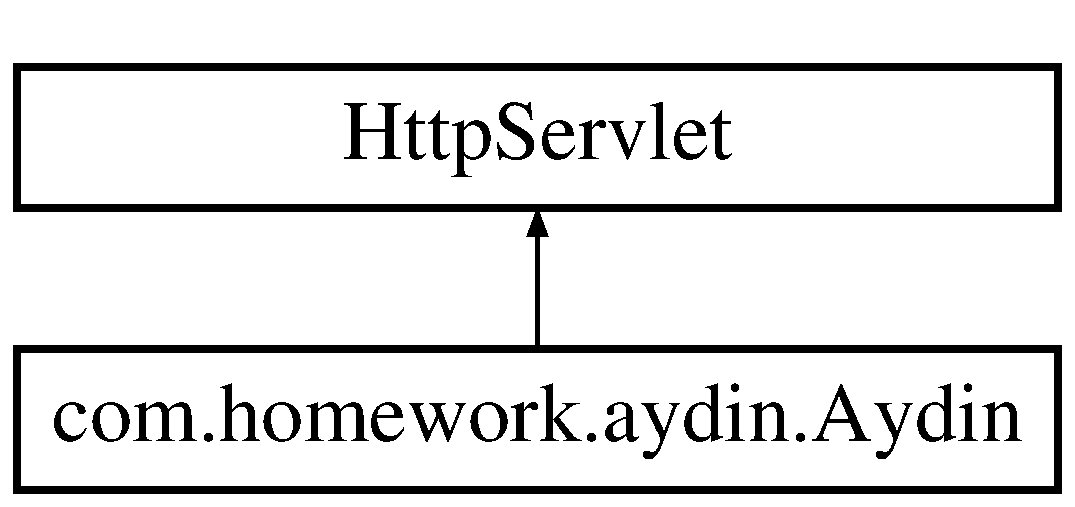
\includegraphics[height=2.000000cm]{classcom_1_1homework_1_1aydin_1_1_aydin}
\end{center}
\end{figure}
\subsection*{Public Member Functions}
\begin{DoxyCompactItemize}
\item 
\hyperlink{classcom_1_1homework_1_1aydin_1_1_aydin_a2ede141d77b6e437e10f3da056d7f116}{Aydin} ()
\end{DoxyCompactItemize}
\subsection*{Protected Member Functions}
\begin{DoxyCompactItemize}
\item 
void \hyperlink{classcom_1_1homework_1_1aydin_1_1_aydin_a307f64d407db1b6402d28ffaea0370a9}{do\+Get} (Http\+Servlet\+Request request, Http\+Servlet\+Response response)  throws Servlet\+Exception, I\+O\+Exception 
\item 
void \hyperlink{classcom_1_1homework_1_1aydin_1_1_aydin_af8469a95252334d3e3b350bcae6e7e1f}{do\+Post} (Http\+Servlet\+Request request, Http\+Servlet\+Response response)  throws Servlet\+Exception, I\+O\+Exception 
\end{DoxyCompactItemize}
\subsection*{Static Private Attributes}
\begin{DoxyCompactItemize}
\item 
static final long \hyperlink{classcom_1_1homework_1_1aydin_1_1_aydin_a36327d610cbc4ac41f7c9f3bf5589f23}{serial\+Version\+U\+ID} = 1L
\end{DoxyCompactItemize}


\subsection{Detailed Description}
Servlet implementation class \hyperlink{classcom_1_1homework_1_1aydin_1_1_aydin}{Aydin} 

\subsection{Constructor \& Destructor Documentation}
\index{com\+::homework\+::aydin\+::\+Aydin@{com\+::homework\+::aydin\+::\+Aydin}!Aydin@{Aydin}}
\index{Aydin@{Aydin}!com\+::homework\+::aydin\+::\+Aydin@{com\+::homework\+::aydin\+::\+Aydin}}
\subsubsection[{\texorpdfstring{Aydin()}{Aydin()}}]{\setlength{\rightskip}{0pt plus 5cm}com.\+homework.\+aydin.\+Aydin.\+Aydin (
\begin{DoxyParamCaption}
{}
\end{DoxyParamCaption}
)}\hypertarget{classcom_1_1homework_1_1aydin_1_1_aydin_a2ede141d77b6e437e10f3da056d7f116}{}\label{classcom_1_1homework_1_1aydin_1_1_aydin_a2ede141d77b6e437e10f3da056d7f116}
\begin{DoxySeeAlso}{See also}
Http\+Servlet\+::\+Http\+Servlet() 
\end{DoxySeeAlso}


\subsection{Member Function Documentation}
\index{com\+::homework\+::aydin\+::\+Aydin@{com\+::homework\+::aydin\+::\+Aydin}!do\+Get@{do\+Get}}
\index{do\+Get@{do\+Get}!com\+::homework\+::aydin\+::\+Aydin@{com\+::homework\+::aydin\+::\+Aydin}}
\subsubsection[{\texorpdfstring{do\+Get(\+Http\+Servlet\+Request request, Http\+Servlet\+Response response)}{doGet(HttpServletRequest request, HttpServletResponse response)}}]{\setlength{\rightskip}{0pt plus 5cm}void com.\+homework.\+aydin.\+Aydin.\+do\+Get (
\begin{DoxyParamCaption}
\item[{Http\+Servlet\+Request}]{request, }
\item[{Http\+Servlet\+Response}]{response}
\end{DoxyParamCaption}
) throws Servlet\+Exception, I\+O\+Exception\hspace{0.3cm}{\ttfamily [protected]}}\hypertarget{classcom_1_1homework_1_1aydin_1_1_aydin_a307f64d407db1b6402d28ffaea0370a9}{}\label{classcom_1_1homework_1_1aydin_1_1_aydin_a307f64d407db1b6402d28ffaea0370a9}
\begin{DoxySeeAlso}{See also}
Http\+Servlet\+::do\+Get(\+Http\+Servlet\+Request request, Http\+Servlet\+Response response) 
\end{DoxySeeAlso}
$<$ Our writer to type html codes \index{com\+::homework\+::aydin\+::\+Aydin@{com\+::homework\+::aydin\+::\+Aydin}!do\+Post@{do\+Post}}
\index{do\+Post@{do\+Post}!com\+::homework\+::aydin\+::\+Aydin@{com\+::homework\+::aydin\+::\+Aydin}}
\subsubsection[{\texorpdfstring{do\+Post(\+Http\+Servlet\+Request request, Http\+Servlet\+Response response)}{doPost(HttpServletRequest request, HttpServletResponse response)}}]{\setlength{\rightskip}{0pt plus 5cm}void com.\+homework.\+aydin.\+Aydin.\+do\+Post (
\begin{DoxyParamCaption}
\item[{Http\+Servlet\+Request}]{request, }
\item[{Http\+Servlet\+Response}]{response}
\end{DoxyParamCaption}
) throws Servlet\+Exception, I\+O\+Exception\hspace{0.3cm}{\ttfamily [protected]}}\hypertarget{classcom_1_1homework_1_1aydin_1_1_aydin_af8469a95252334d3e3b350bcae6e7e1f}{}\label{classcom_1_1homework_1_1aydin_1_1_aydin_af8469a95252334d3e3b350bcae6e7e1f}
\begin{DoxySeeAlso}{See also}
Http\+Servlet\+::do\+Post(\+Http\+Servlet\+Request request, Http\+Servlet\+Response response) 
\end{DoxySeeAlso}


\subsection{Member Data Documentation}
\index{com\+::homework\+::aydin\+::\+Aydin@{com\+::homework\+::aydin\+::\+Aydin}!serial\+Version\+U\+ID@{serial\+Version\+U\+ID}}
\index{serial\+Version\+U\+ID@{serial\+Version\+U\+ID}!com\+::homework\+::aydin\+::\+Aydin@{com\+::homework\+::aydin\+::\+Aydin}}
\subsubsection[{\texorpdfstring{serial\+Version\+U\+ID}{serialVersionUID}}]{\setlength{\rightskip}{0pt plus 5cm}final long com.\+homework.\+aydin.\+Aydin.\+serial\+Version\+U\+ID = 1L\hspace{0.3cm}{\ttfamily [static]}, {\ttfamily [private]}}\hypertarget{classcom_1_1homework_1_1aydin_1_1_aydin_a36327d610cbc4ac41f7c9f3bf5589f23}{}\label{classcom_1_1homework_1_1aydin_1_1_aydin_a36327d610cbc4ac41f7c9f3bf5589f23}


The documentation for this class was generated from the following file\+:\begin{DoxyCompactItemize}
\item 
src/com/homework/aydin/\hyperlink{_aydin_8java}{Aydin.\+java}\end{DoxyCompactItemize}

\hypertarget{classcom_1_1homework_1_1aydin_1_1_d_b_aydin}{}\section{com.\+homework.\+aydin.\+D\+B\+Aydin Class Reference}
\label{classcom_1_1homework_1_1aydin_1_1_d_b_aydin}\index{com.\+homework.\+aydin.\+D\+B\+Aydin@{com.\+homework.\+aydin.\+D\+B\+Aydin}}
\subsection*{Public Member Functions}
\begin{DoxyCompactItemize}
\item 
\hyperlink{classcom_1_1homework_1_1aydin_1_1_d_b_aydin_a153864fa5798ba91fba168de198a797d}{D\+B\+Aydin} (String db\+Name, String username, String password)
\item 
Connection \hyperlink{classcom_1_1homework_1_1aydin_1_1_d_b_aydin_aa54ee4985e5a6b99af7606f829d438a9}{get\+Connection} ()
\item 
void \hyperlink{classcom_1_1homework_1_1aydin_1_1_d_b_aydin_a285721a7c0b3ed8dbfc2086cf47e82b5}{init} (Vector$<$ \hyperlink{classcom_1_1homework_1_1aydin_1_1_model_aydin}{Model\+Aydin} $>$ pre\+Data)
\item 
void \hyperlink{classcom_1_1homework_1_1aydin_1_1_d_b_aydin_a9aba7b406829dd700791d0c4399926be}{delete} ()
\item 
Vector$<$ \hyperlink{classcom_1_1homework_1_1aydin_1_1_model_aydin}{Model\+Aydin} $>$ \hyperlink{classcom_1_1homework_1_1aydin_1_1_d_b_aydin_aa7970348bbf02052742008b04cdf013e}{search} (String parameter)
\end{DoxyCompactItemize}


\subsection{Constructor \& Destructor Documentation}
\index{com\+::homework\+::aydin\+::\+D\+B\+Aydin@{com\+::homework\+::aydin\+::\+D\+B\+Aydin}!D\+B\+Aydin@{D\+B\+Aydin}}
\index{D\+B\+Aydin@{D\+B\+Aydin}!com\+::homework\+::aydin\+::\+D\+B\+Aydin@{com\+::homework\+::aydin\+::\+D\+B\+Aydin}}
\subsubsection[{\texorpdfstring{D\+B\+Aydin(\+String db\+Name, String username, String password)}{DBAydin(String dbName, String username, String password)}}]{\setlength{\rightskip}{0pt plus 5cm}com.\+homework.\+aydin.\+D\+B\+Aydin.\+D\+B\+Aydin (
\begin{DoxyParamCaption}
\item[{String}]{db\+Name, }
\item[{String}]{username, }
\item[{String}]{password}
\end{DoxyParamCaption}
)}\hypertarget{classcom_1_1homework_1_1aydin_1_1_d_b_aydin_a153864fa5798ba91fba168de198a797d}{}\label{classcom_1_1homework_1_1aydin_1_1_d_b_aydin_a153864fa5798ba91fba168de198a797d}


\subsection{Member Function Documentation}
\index{com\+::homework\+::aydin\+::\+D\+B\+Aydin@{com\+::homework\+::aydin\+::\+D\+B\+Aydin}!delete@{delete}}
\index{delete@{delete}!com\+::homework\+::aydin\+::\+D\+B\+Aydin@{com\+::homework\+::aydin\+::\+D\+B\+Aydin}}
\subsubsection[{\texorpdfstring{delete()}{delete()}}]{\setlength{\rightskip}{0pt plus 5cm}void com.\+homework.\+aydin.\+D\+B\+Aydin.\+delete (
\begin{DoxyParamCaption}
{}
\end{DoxyParamCaption}
)}\hypertarget{classcom_1_1homework_1_1aydin_1_1_d_b_aydin_a9aba7b406829dd700791d0c4399926be}{}\label{classcom_1_1homework_1_1aydin_1_1_d_b_aydin_a9aba7b406829dd700791d0c4399926be}
\index{com\+::homework\+::aydin\+::\+D\+B\+Aydin@{com\+::homework\+::aydin\+::\+D\+B\+Aydin}!get\+Connection@{get\+Connection}}
\index{get\+Connection@{get\+Connection}!com\+::homework\+::aydin\+::\+D\+B\+Aydin@{com\+::homework\+::aydin\+::\+D\+B\+Aydin}}
\subsubsection[{\texorpdfstring{get\+Connection()}{getConnection()}}]{\setlength{\rightskip}{0pt plus 5cm}Connection com.\+homework.\+aydin.\+D\+B\+Aydin.\+get\+Connection (
\begin{DoxyParamCaption}
{}
\end{DoxyParamCaption}
)}\hypertarget{classcom_1_1homework_1_1aydin_1_1_d_b_aydin_aa54ee4985e5a6b99af7606f829d438a9}{}\label{classcom_1_1homework_1_1aydin_1_1_d_b_aydin_aa54ee4985e5a6b99af7606f829d438a9}
\index{com\+::homework\+::aydin\+::\+D\+B\+Aydin@{com\+::homework\+::aydin\+::\+D\+B\+Aydin}!init@{init}}
\index{init@{init}!com\+::homework\+::aydin\+::\+D\+B\+Aydin@{com\+::homework\+::aydin\+::\+D\+B\+Aydin}}
\subsubsection[{\texorpdfstring{init(\+Vector$<$ Model\+Aydin $>$ pre\+Data)}{init(Vector< ModelAydin > preData)}}]{\setlength{\rightskip}{0pt plus 5cm}void com.\+homework.\+aydin.\+D\+B\+Aydin.\+init (
\begin{DoxyParamCaption}
\item[{Vector$<$ {\bf Model\+Aydin} $>$}]{pre\+Data}
\end{DoxyParamCaption}
)}\hypertarget{classcom_1_1homework_1_1aydin_1_1_d_b_aydin_a285721a7c0b3ed8dbfc2086cf47e82b5}{}\label{classcom_1_1homework_1_1aydin_1_1_d_b_aydin_a285721a7c0b3ed8dbfc2086cf47e82b5}
\index{com\+::homework\+::aydin\+::\+D\+B\+Aydin@{com\+::homework\+::aydin\+::\+D\+B\+Aydin}!search@{search}}
\index{search@{search}!com\+::homework\+::aydin\+::\+D\+B\+Aydin@{com\+::homework\+::aydin\+::\+D\+B\+Aydin}}
\subsubsection[{\texorpdfstring{search(\+String parameter)}{search(String parameter)}}]{\setlength{\rightskip}{0pt plus 5cm}Vector$<${\bf Model\+Aydin}$>$ com.\+homework.\+aydin.\+D\+B\+Aydin.\+search (
\begin{DoxyParamCaption}
\item[{String}]{parameter}
\end{DoxyParamCaption}
)}\hypertarget{classcom_1_1homework_1_1aydin_1_1_d_b_aydin_aa7970348bbf02052742008b04cdf013e}{}\label{classcom_1_1homework_1_1aydin_1_1_d_b_aydin_aa7970348bbf02052742008b04cdf013e}


The documentation for this class was generated from the following file\+:\begin{DoxyCompactItemize}
\item 
src/com/homework/aydin/\hyperlink{_d_b_aydin_8java}{D\+B\+Aydin.\+java}\end{DoxyCompactItemize}

\hypertarget{classcom_1_1homework_1_1denizalp_1_1_db_denizalp}{}\section{com.\+homework.\+denizalp.\+Db\+Denizalp Class Reference}
\label{classcom_1_1homework_1_1denizalp_1_1_db_denizalp}\index{com.\+homework.\+denizalp.\+Db\+Denizalp@{com.\+homework.\+denizalp.\+Db\+Denizalp}}
\subsection*{Public Member Functions}
\begin{DoxyCompactItemize}
\item 
\hyperlink{classcom_1_1homework_1_1denizalp_1_1_db_denizalp_a55810e1c3e29b25d6490d0be66173f8d}{Db\+Denizalp} (String db\+Name, String username, String password)
\item 
Connection \hyperlink{classcom_1_1homework_1_1denizalp_1_1_db_denizalp_a112da3b6326345251be868362ad28438}{get\+Connection} ()
\end{DoxyCompactItemize}


\subsection{Constructor \& Destructor Documentation}
\index{com\+::homework\+::denizalp\+::\+Db\+Denizalp@{com\+::homework\+::denizalp\+::\+Db\+Denizalp}!Db\+Denizalp@{Db\+Denizalp}}
\index{Db\+Denizalp@{Db\+Denizalp}!com\+::homework\+::denizalp\+::\+Db\+Denizalp@{com\+::homework\+::denizalp\+::\+Db\+Denizalp}}
\subsubsection[{\texorpdfstring{Db\+Denizalp(\+String db\+Name, String username, String password)}{DbDenizalp(String dbName, String username, String password)}}]{\setlength{\rightskip}{0pt plus 5cm}com.\+homework.\+denizalp.\+Db\+Denizalp.\+Db\+Denizalp (
\begin{DoxyParamCaption}
\item[{String}]{db\+Name, }
\item[{String}]{username, }
\item[{String}]{password}
\end{DoxyParamCaption}
)}\hypertarget{classcom_1_1homework_1_1denizalp_1_1_db_denizalp_a55810e1c3e29b25d6490d0be66173f8d}{}\label{classcom_1_1homework_1_1denizalp_1_1_db_denizalp_a55810e1c3e29b25d6490d0be66173f8d}


\subsection{Member Function Documentation}
\index{com\+::homework\+::denizalp\+::\+Db\+Denizalp@{com\+::homework\+::denizalp\+::\+Db\+Denizalp}!get\+Connection@{get\+Connection}}
\index{get\+Connection@{get\+Connection}!com\+::homework\+::denizalp\+::\+Db\+Denizalp@{com\+::homework\+::denizalp\+::\+Db\+Denizalp}}
\subsubsection[{\texorpdfstring{get\+Connection()}{getConnection()}}]{\setlength{\rightskip}{0pt plus 5cm}Connection com.\+homework.\+denizalp.\+Db\+Denizalp.\+get\+Connection (
\begin{DoxyParamCaption}
{}
\end{DoxyParamCaption}
)}\hypertarget{classcom_1_1homework_1_1denizalp_1_1_db_denizalp_a112da3b6326345251be868362ad28438}{}\label{classcom_1_1homework_1_1denizalp_1_1_db_denizalp_a112da3b6326345251be868362ad28438}


The documentation for this class was generated from the following file\+:\begin{DoxyCompactItemize}
\item 
src/com/homework/denizalp/\hyperlink{_db_denizalp_8java}{Db\+Denizalp.\+java}\end{DoxyCompactItemize}

\hypertarget{classcom_1_1homework_1_1yunus_1_1_db_yunus}{}\section{com.\+homework.\+yunus.\+Db\+Yunus Class Reference}
\label{classcom_1_1homework_1_1yunus_1_1_db_yunus}\index{com.\+homework.\+yunus.\+Db\+Yunus@{com.\+homework.\+yunus.\+Db\+Yunus}}
\subsection*{Public Member Functions}
\begin{DoxyCompactItemize}
\item 
\hyperlink{classcom_1_1homework_1_1yunus_1_1_db_yunus_a0471eb6b18272009f3bd3728510f4c6c}{Db\+Yunus} (String db\+Name, String username, String password)
\item 
Connection \hyperlink{classcom_1_1homework_1_1yunus_1_1_db_yunus_a5cdbf15a8027a2d8ff2201d451e12297}{get\+Connection} ()
\item 
void \hyperlink{classcom_1_1homework_1_1yunus_1_1_db_yunus_af545ad91b2ddf224346cb4914bd36583}{init} (Vector$<$ \hyperlink{classcom_1_1homework_1_1yunus_1_1_model_yunus}{Model\+Yunus} $>$ data)
\item 
void \hyperlink{classcom_1_1homework_1_1yunus_1_1_db_yunus_ac0f46ce9c1b762a530e4f19fae4e0f01}{delete} ()
\item 
Vector$<$ \hyperlink{classcom_1_1homework_1_1yunus_1_1_model_yunus}{Model\+Yunus} $>$ \hyperlink{classcom_1_1homework_1_1yunus_1_1_db_yunus_a3010b549e3a1b7b21d63c65f66d5a7eb}{search} (String str)
\item 
void \hyperlink{classcom_1_1homework_1_1yunus_1_1_db_yunus_a36c0889028f98b4c5d823f17c3efbd71}{save\+Search} (String timestamp, String query, String selecteditems)
\item 
String \hyperlink{classcom_1_1homework_1_1yunus_1_1_db_yunus_a35f377c750efbe182daa17daaf9af672}{get\+History} ()
\end{DoxyCompactItemize}


\subsection{Detailed Description}
Database Layer of \hyperlink{classcom_1_1homework_1_1yunus_1_1_yunus}{Yunus} package. This class uses jdbc mysql connector library under webapp libs \begin{DoxyAuthor}{Author}
\hyperlink{classcom_1_1homework_1_1yunus_1_1_yunus}{Yunus} 
\end{DoxyAuthor}


\subsection{Constructor \& Destructor Documentation}
\index{com\+::homework\+::yunus\+::\+Db\+Yunus@{com\+::homework\+::yunus\+::\+Db\+Yunus}!Db\+Yunus@{Db\+Yunus}}
\index{Db\+Yunus@{Db\+Yunus}!com\+::homework\+::yunus\+::\+Db\+Yunus@{com\+::homework\+::yunus\+::\+Db\+Yunus}}
\subsubsection[{\texorpdfstring{Db\+Yunus(\+String db\+Name, String username, String password)}{DbYunus(String dbName, String username, String password)}}]{\setlength{\rightskip}{0pt plus 5cm}com.\+homework.\+yunus.\+Db\+Yunus.\+Db\+Yunus (
\begin{DoxyParamCaption}
\item[{String}]{db\+Name, }
\item[{String}]{username, }
\item[{String}]{password}
\end{DoxyParamCaption}
)}\hypertarget{classcom_1_1homework_1_1yunus_1_1_db_yunus_a0471eb6b18272009f3bd3728510f4c6c}{}\label{classcom_1_1homework_1_1yunus_1_1_db_yunus_a0471eb6b18272009f3bd3728510f4c6c}

\begin{DoxyParams}{Parameters}
{\em db\+Name} & User\textquotesingle{}s personal database name \\
\hline
{\em username} & Mysql server username \\
\hline
{\em password} & Mysql server password \\
\hline
\end{DoxyParams}


\subsection{Member Function Documentation}
\index{com\+::homework\+::yunus\+::\+Db\+Yunus@{com\+::homework\+::yunus\+::\+Db\+Yunus}!delete@{delete}}
\index{delete@{delete}!com\+::homework\+::yunus\+::\+Db\+Yunus@{com\+::homework\+::yunus\+::\+Db\+Yunus}}
\subsubsection[{\texorpdfstring{delete()}{delete()}}]{\setlength{\rightskip}{0pt plus 5cm}void com.\+homework.\+yunus.\+Db\+Yunus.\+delete (
\begin{DoxyParamCaption}
{}
\end{DoxyParamCaption}
)}\hypertarget{classcom_1_1homework_1_1yunus_1_1_db_yunus_ac0f46ce9c1b762a530e4f19fae4e0f01}{}\label{classcom_1_1homework_1_1yunus_1_1_db_yunus_ac0f46ce9c1b762a530e4f19fae4e0f01}
Deletes all data on the table to reset the database. Initialization is usually used after this method. \index{com\+::homework\+::yunus\+::\+Db\+Yunus@{com\+::homework\+::yunus\+::\+Db\+Yunus}!get\+Connection@{get\+Connection}}
\index{get\+Connection@{get\+Connection}!com\+::homework\+::yunus\+::\+Db\+Yunus@{com\+::homework\+::yunus\+::\+Db\+Yunus}}
\subsubsection[{\texorpdfstring{get\+Connection()}{getConnection()}}]{\setlength{\rightskip}{0pt plus 5cm}Connection com.\+homework.\+yunus.\+Db\+Yunus.\+get\+Connection (
\begin{DoxyParamCaption}
{}
\end{DoxyParamCaption}
)}\hypertarget{classcom_1_1homework_1_1yunus_1_1_db_yunus_a5cdbf15a8027a2d8ff2201d451e12297}{}\label{classcom_1_1homework_1_1yunus_1_1_db_yunus_a5cdbf15a8027a2d8ff2201d451e12297}
After constructing the connection, Servlet can get connection by this method \begin{DoxyReturn}{Returns}
Not Null connection 
\end{DoxyReturn}
\index{com\+::homework\+::yunus\+::\+Db\+Yunus@{com\+::homework\+::yunus\+::\+Db\+Yunus}!get\+History@{get\+History}}
\index{get\+History@{get\+History}!com\+::homework\+::yunus\+::\+Db\+Yunus@{com\+::homework\+::yunus\+::\+Db\+Yunus}}
\subsubsection[{\texorpdfstring{get\+History()}{getHistory()}}]{\setlength{\rightskip}{0pt plus 5cm}String com.\+homework.\+yunus.\+Db\+Yunus.\+get\+History (
\begin{DoxyParamCaption}
{}
\end{DoxyParamCaption}
)}\hypertarget{classcom_1_1homework_1_1yunus_1_1_db_yunus_a35f377c750efbe182daa17daaf9af672}{}\label{classcom_1_1homework_1_1yunus_1_1_db_yunus_a35f377c750efbe182daa17daaf9af672}
Selects the history from database Converts it to a html format that can be written as a string \begin{DoxyReturn}{Returns}
History data as String 
\end{DoxyReturn}
\index{com\+::homework\+::yunus\+::\+Db\+Yunus@{com\+::homework\+::yunus\+::\+Db\+Yunus}!init@{init}}
\index{init@{init}!com\+::homework\+::yunus\+::\+Db\+Yunus@{com\+::homework\+::yunus\+::\+Db\+Yunus}}
\subsubsection[{\texorpdfstring{init(\+Vector$<$ Model\+Yunus $>$ data)}{init(Vector< ModelYunus > data)}}]{\setlength{\rightskip}{0pt plus 5cm}void com.\+homework.\+yunus.\+Db\+Yunus.\+init (
\begin{DoxyParamCaption}
\item[{Vector$<$ {\bf Model\+Yunus} $>$}]{data}
\end{DoxyParamCaption}
)}\hypertarget{classcom_1_1homework_1_1yunus_1_1_db_yunus_af545ad91b2ddf224346cb4914bd36583}{}\label{classcom_1_1homework_1_1yunus_1_1_db_yunus_af545ad91b2ddf224346cb4914bd36583}
Initializes the database to given data list from sparql query result. 
\begin{DoxyParams}{Parameters}
{\em data} & parsed and modeled data that comes from sparql query result \\
\hline
\end{DoxyParams}
\index{com\+::homework\+::yunus\+::\+Db\+Yunus@{com\+::homework\+::yunus\+::\+Db\+Yunus}!save\+Search@{save\+Search}}
\index{save\+Search@{save\+Search}!com\+::homework\+::yunus\+::\+Db\+Yunus@{com\+::homework\+::yunus\+::\+Db\+Yunus}}
\subsubsection[{\texorpdfstring{save\+Search(\+String timestamp, String query, String selecteditems)}{saveSearch(String timestamp, String query, String selecteditems)}}]{\setlength{\rightskip}{0pt plus 5cm}void com.\+homework.\+yunus.\+Db\+Yunus.\+save\+Search (
\begin{DoxyParamCaption}
\item[{String}]{timestamp, }
\item[{String}]{query, }
\item[{String}]{selecteditems}
\end{DoxyParamCaption}
)}\hypertarget{classcom_1_1homework_1_1yunus_1_1_db_yunus_a36c0889028f98b4c5d823f17c3efbd71}{}\label{classcom_1_1homework_1_1yunus_1_1_db_yunus_a36c0889028f98b4c5d823f17c3efbd71}
Saves selected data to database with timestamp of the search and query 
\begin{DoxyParams}{Parameters}
{\em timestamp} & time that search is made \\
\hline
{\em query} & query that is searched \\
\hline
{\em selecteditems} & number of rows that selected \\
\hline
\end{DoxyParams}
\index{com\+::homework\+::yunus\+::\+Db\+Yunus@{com\+::homework\+::yunus\+::\+Db\+Yunus}!search@{search}}
\index{search@{search}!com\+::homework\+::yunus\+::\+Db\+Yunus@{com\+::homework\+::yunus\+::\+Db\+Yunus}}
\subsubsection[{\texorpdfstring{search(\+String str)}{search(String str)}}]{\setlength{\rightskip}{0pt plus 5cm}Vector$<${\bf Model\+Yunus}$>$ com.\+homework.\+yunus.\+Db\+Yunus.\+search (
\begin{DoxyParamCaption}
\item[{String}]{str}
\end{DoxyParamCaption}
)}\hypertarget{classcom_1_1homework_1_1yunus_1_1_db_yunus_a3010b549e3a1b7b21d63c65f66d5a7eb}{}\label{classcom_1_1homework_1_1yunus_1_1_db_yunus_a3010b549e3a1b7b21d63c65f66d5a7eb}
According to given input string, searches the query on database on returns parsed Model data as a list 
\begin{DoxyParams}{Parameters}
{\em str} & Country name \\
\hline
\end{DoxyParams}
\begin{DoxyReturn}{Returns}
data that is the result of the search 
\end{DoxyReturn}


The documentation for this class was generated from the following file\+:\begin{DoxyCompactItemize}
\item 
src/com/homework/yunus/\hyperlink{_db_yunus_8java}{Db\+Yunus.\+java}\end{DoxyCompactItemize}

\hypertarget{classcom_1_1homework_1_1denizalp_1_1_denizalp}{}\section{com.\+homework.\+denizalp.\+Denizalp Class Reference}
\label{classcom_1_1homework_1_1denizalp_1_1_denizalp}\index{com.\+homework.\+denizalp.\+Denizalp@{com.\+homework.\+denizalp.\+Denizalp}}
Inheritance diagram for com.\+homework.\+denizalp.\+Denizalp\+:\begin{figure}[H]
\begin{center}
\leavevmode
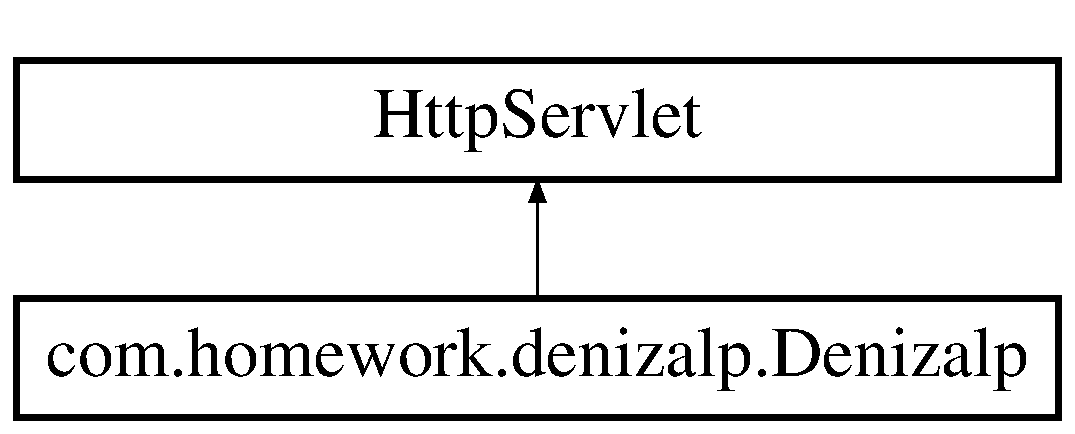
\includegraphics[height=2.000000cm]{classcom_1_1homework_1_1denizalp_1_1_denizalp}
\end{center}
\end{figure}
\subsection*{Public Member Functions}
\begin{DoxyCompactItemize}
\item 
\hyperlink{classcom_1_1homework_1_1denizalp_1_1_denizalp_ae15225067faa1f6a5a42555e8e46d98e}{Denizalp} ()
\end{DoxyCompactItemize}
\subsection*{Protected Member Functions}
\begin{DoxyCompactItemize}
\item 
void \hyperlink{classcom_1_1homework_1_1denizalp_1_1_denizalp_a5ceb5e4e159bae7b8486d97db7ac8379}{do\+Get} (Http\+Servlet\+Request request, Http\+Servlet\+Response response)  throws Servlet\+Exception, I\+O\+Exception 
\end{DoxyCompactItemize}
\subsection*{Static Private Attributes}
\begin{DoxyCompactItemize}
\item 
static final long \hyperlink{classcom_1_1homework_1_1denizalp_1_1_denizalp_a0ba32279227f2b418ea1da8996859de8}{serial\+Version\+U\+ID} = 1L
\end{DoxyCompactItemize}


\subsection{Detailed Description}
Servlet implementation class \hyperlink{classcom_1_1homework_1_1denizalp_1_1_denizalp}{Denizalp} connects to database 

\subsection{Constructor \& Destructor Documentation}
\index{com\+::homework\+::denizalp\+::\+Denizalp@{com\+::homework\+::denizalp\+::\+Denizalp}!Denizalp@{Denizalp}}
\index{Denizalp@{Denizalp}!com\+::homework\+::denizalp\+::\+Denizalp@{com\+::homework\+::denizalp\+::\+Denizalp}}
\subsubsection[{\texorpdfstring{Denizalp()}{Denizalp()}}]{\setlength{\rightskip}{0pt plus 5cm}com.\+homework.\+denizalp.\+Denizalp.\+Denizalp (
\begin{DoxyParamCaption}
{}
\end{DoxyParamCaption}
)}\hypertarget{classcom_1_1homework_1_1denizalp_1_1_denizalp_ae15225067faa1f6a5a42555e8e46d98e}{}\label{classcom_1_1homework_1_1denizalp_1_1_denizalp_ae15225067faa1f6a5a42555e8e46d98e}
\begin{DoxySeeAlso}{See also}
Http\+Servlet\+::\+Http\+Servlet() 
\end{DoxySeeAlso}


\subsection{Member Function Documentation}
\index{com\+::homework\+::denizalp\+::\+Denizalp@{com\+::homework\+::denizalp\+::\+Denizalp}!do\+Get@{do\+Get}}
\index{do\+Get@{do\+Get}!com\+::homework\+::denizalp\+::\+Denizalp@{com\+::homework\+::denizalp\+::\+Denizalp}}
\subsubsection[{\texorpdfstring{do\+Get(\+Http\+Servlet\+Request request, Http\+Servlet\+Response response)}{doGet(HttpServletRequest request, HttpServletResponse response)}}]{\setlength{\rightskip}{0pt plus 5cm}void com.\+homework.\+denizalp.\+Denizalp.\+do\+Get (
\begin{DoxyParamCaption}
\item[{Http\+Servlet\+Request}]{request, }
\item[{Http\+Servlet\+Response}]{response}
\end{DoxyParamCaption}
) throws Servlet\+Exception, I\+O\+Exception\hspace{0.3cm}{\ttfamily [protected]}}\hypertarget{classcom_1_1homework_1_1denizalp_1_1_denizalp_a5ceb5e4e159bae7b8486d97db7ac8379}{}\label{classcom_1_1homework_1_1denizalp_1_1_denizalp_a5ceb5e4e159bae7b8486d97db7ac8379}
\begin{DoxySeeAlso}{See also}
Http\+Servlet\+::do\+Get(\+Http\+Servlet\+Request request, Http\+Servlet\+Response response) 
\end{DoxySeeAlso}
$<$ Our writer to type html codes

$<$ database connection variable 

\subsection{Member Data Documentation}
\index{com\+::homework\+::denizalp\+::\+Denizalp@{com\+::homework\+::denizalp\+::\+Denizalp}!serial\+Version\+U\+ID@{serial\+Version\+U\+ID}}
\index{serial\+Version\+U\+ID@{serial\+Version\+U\+ID}!com\+::homework\+::denizalp\+::\+Denizalp@{com\+::homework\+::denizalp\+::\+Denizalp}}
\subsubsection[{\texorpdfstring{serial\+Version\+U\+ID}{serialVersionUID}}]{\setlength{\rightskip}{0pt plus 5cm}final long com.\+homework.\+denizalp.\+Denizalp.\+serial\+Version\+U\+ID = 1L\hspace{0.3cm}{\ttfamily [static]}, {\ttfamily [private]}}\hypertarget{classcom_1_1homework_1_1denizalp_1_1_denizalp_a0ba32279227f2b418ea1da8996859de8}{}\label{classcom_1_1homework_1_1denizalp_1_1_denizalp_a0ba32279227f2b418ea1da8996859de8}


The documentation for this class was generated from the following file\+:\begin{DoxyCompactItemize}
\item 
src/com/homework/denizalp/\hyperlink{_denizalp_8java}{Denizalp.\+java}\end{DoxyCompactItemize}

\hypertarget{classcom_1_1homework_1_1home_1_1_home}{}\section{com.\+homework.\+home.\+Home Class Reference}
\label{classcom_1_1homework_1_1home_1_1_home}\index{com.\+homework.\+home.\+Home@{com.\+homework.\+home.\+Home}}
Inheritance diagram for com.\+homework.\+home.\+Home\+:\begin{figure}[H]
\begin{center}
\leavevmode
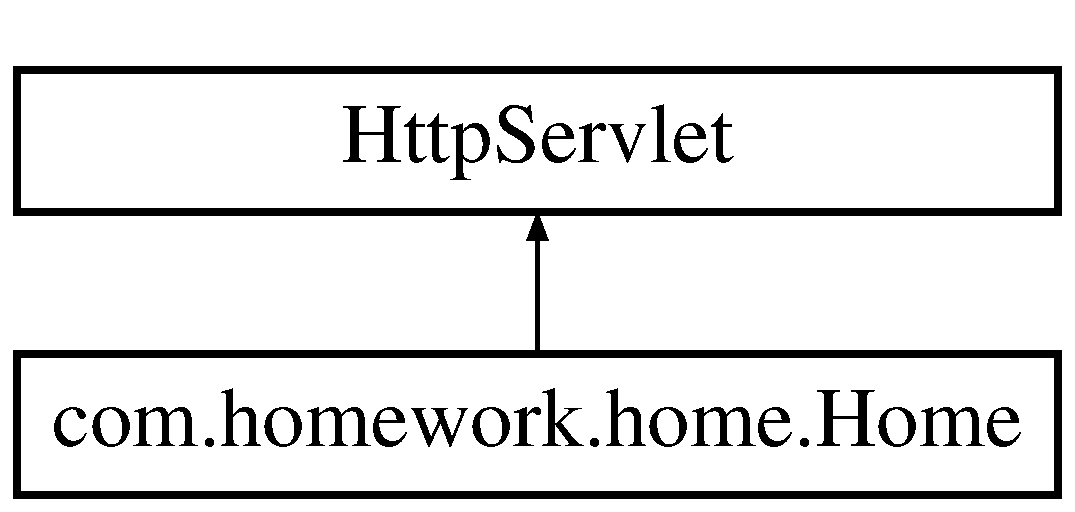
\includegraphics[height=2.000000cm]{classcom_1_1homework_1_1home_1_1_home}
\end{center}
\end{figure}
\subsection*{Public Member Functions}
\begin{DoxyCompactItemize}
\item 
\hyperlink{classcom_1_1homework_1_1home_1_1_home_ac5127b125cf55fbef4e84aaf0728fd72}{Home} ()
\end{DoxyCompactItemize}
\subsection*{Protected Member Functions}
\begin{DoxyCompactItemize}
\item 
void \hyperlink{classcom_1_1homework_1_1home_1_1_home_a390ad06ac932e0ab47bcad1469c9c174}{do\+Get} (Http\+Servlet\+Request request, Http\+Servlet\+Response response)  throws Servlet\+Exception, I\+O\+Exception 
\end{DoxyCompactItemize}
\subsection*{Static Private Attributes}
\begin{DoxyCompactItemize}
\item 
static final long \hyperlink{classcom_1_1homework_1_1home_1_1_home_ab7840589e7705ec054b07f9488dc9b4e}{serial\+Version\+U\+ID} = 1L
\end{DoxyCompactItemize}


\subsection{Constructor \& Destructor Documentation}
\index{com\+::homework\+::home\+::\+Home@{com\+::homework\+::home\+::\+Home}!Home@{Home}}
\index{Home@{Home}!com\+::homework\+::home\+::\+Home@{com\+::homework\+::home\+::\+Home}}
\subsubsection[{\texorpdfstring{Home()}{Home()}}]{\setlength{\rightskip}{0pt plus 5cm}com.\+homework.\+home.\+Home.\+Home (
\begin{DoxyParamCaption}
{}
\end{DoxyParamCaption}
)}\hypertarget{classcom_1_1homework_1_1home_1_1_home_ac5127b125cf55fbef4e84aaf0728fd72}{}\label{classcom_1_1homework_1_1home_1_1_home_ac5127b125cf55fbef4e84aaf0728fd72}


\subsection{Member Function Documentation}
\index{com\+::homework\+::home\+::\+Home@{com\+::homework\+::home\+::\+Home}!do\+Get@{do\+Get}}
\index{do\+Get@{do\+Get}!com\+::homework\+::home\+::\+Home@{com\+::homework\+::home\+::\+Home}}
\subsubsection[{\texorpdfstring{do\+Get(\+Http\+Servlet\+Request request, Http\+Servlet\+Response response)}{doGet(HttpServletRequest request, HttpServletResponse response)}}]{\setlength{\rightskip}{0pt plus 5cm}void com.\+homework.\+home.\+Home.\+do\+Get (
\begin{DoxyParamCaption}
\item[{Http\+Servlet\+Request}]{request, }
\item[{Http\+Servlet\+Response}]{response}
\end{DoxyParamCaption}
) throws Servlet\+Exception, I\+O\+Exception\hspace{0.3cm}{\ttfamily [protected]}}\hypertarget{classcom_1_1homework_1_1home_1_1_home_a390ad06ac932e0ab47bcad1469c9c174}{}\label{classcom_1_1homework_1_1home_1_1_home_a390ad06ac932e0ab47bcad1469c9c174}


\subsection{Member Data Documentation}
\index{com\+::homework\+::home\+::\+Home@{com\+::homework\+::home\+::\+Home}!serial\+Version\+U\+ID@{serial\+Version\+U\+ID}}
\index{serial\+Version\+U\+ID@{serial\+Version\+U\+ID}!com\+::homework\+::home\+::\+Home@{com\+::homework\+::home\+::\+Home}}
\subsubsection[{\texorpdfstring{serial\+Version\+U\+ID}{serialVersionUID}}]{\setlength{\rightskip}{0pt plus 5cm}final long com.\+homework.\+home.\+Home.\+serial\+Version\+U\+ID = 1L\hspace{0.3cm}{\ttfamily [static]}, {\ttfamily [private]}}\hypertarget{classcom_1_1homework_1_1home_1_1_home_ab7840589e7705ec054b07f9488dc9b4e}{}\label{classcom_1_1homework_1_1home_1_1_home_ab7840589e7705ec054b07f9488dc9b4e}


The documentation for this class was generated from the following file\+:\begin{DoxyCompactItemize}
\item 
src/com/homework/home/\hyperlink{_home_8java}{Home.\+java}\end{DoxyCompactItemize}

\hypertarget{classcom_1_1homework_1_1kubra_1_1_kubra}{}\section{com.\+homework.\+kubra.\+Kubra Class Reference}
\label{classcom_1_1homework_1_1kubra_1_1_kubra}\index{com.\+homework.\+kubra.\+Kubra@{com.\+homework.\+kubra.\+Kubra}}
Inheritance diagram for com.\+homework.\+kubra.\+Kubra\+:\begin{figure}[H]
\begin{center}
\leavevmode
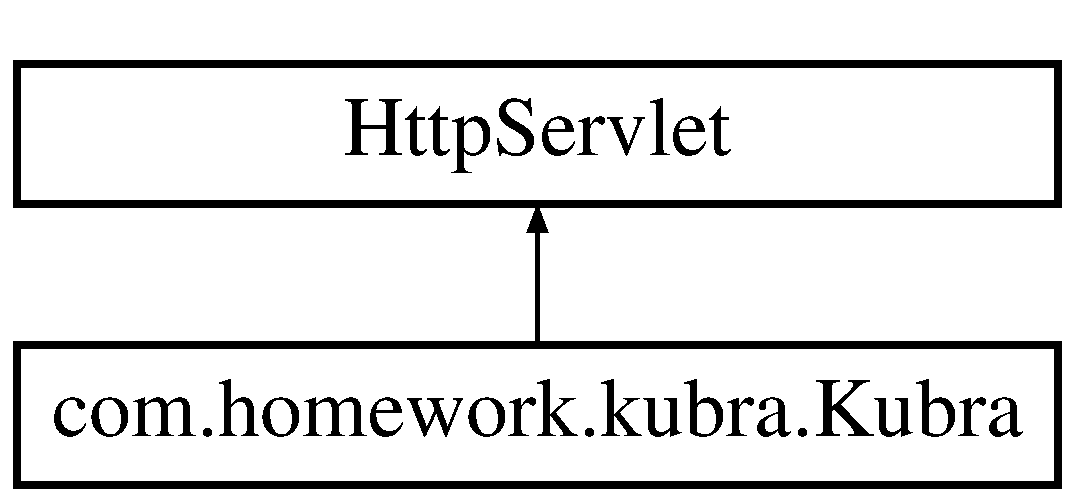
\includegraphics[height=2.000000cm]{classcom_1_1homework_1_1kubra_1_1_kubra}
\end{center}
\end{figure}
\subsection*{Public Member Functions}
\begin{DoxyCompactItemize}
\item 
\hyperlink{classcom_1_1homework_1_1kubra_1_1_kubra_a426ba02e54e1b29f0faad26c3445c4f5}{Kubra} ()
\end{DoxyCompactItemize}
\subsection*{Protected Member Functions}
\begin{DoxyCompactItemize}
\item 
void \hyperlink{classcom_1_1homework_1_1kubra_1_1_kubra_ac848be3c477ee3497de96a7da7143537}{do\+Get} (Http\+Servlet\+Request request, Http\+Servlet\+Response response)  throws Servlet\+Exception, I\+O\+Exception 
\item 
void \hyperlink{classcom_1_1homework_1_1kubra_1_1_kubra_abd450e07b8b3abb94cd768c12727cf51}{do\+Post} (Http\+Servlet\+Request req, Http\+Servlet\+Response resp)  throws Servlet\+Exception, I\+O\+Exception 
\end{DoxyCompactItemize}
\subsection*{Static Private Attributes}
\begin{DoxyCompactItemize}
\item 
static final long \hyperlink{classcom_1_1homework_1_1kubra_1_1_kubra_a2eb40523c9e5223c53add8d16cc9ac0e}{serial\+Version\+U\+ID} = 1L
\end{DoxyCompactItemize}


\subsection{Constructor \& Destructor Documentation}
\index{com\+::homework\+::kubra\+::\+Kubra@{com\+::homework\+::kubra\+::\+Kubra}!Kubra@{Kubra}}
\index{Kubra@{Kubra}!com\+::homework\+::kubra\+::\+Kubra@{com\+::homework\+::kubra\+::\+Kubra}}
\subsubsection[{\texorpdfstring{Kubra()}{Kubra()}}]{\setlength{\rightskip}{0pt plus 5cm}com.\+homework.\+kubra.\+Kubra.\+Kubra (
\begin{DoxyParamCaption}
{}
\end{DoxyParamCaption}
)}\hypertarget{classcom_1_1homework_1_1kubra_1_1_kubra_a426ba02e54e1b29f0faad26c3445c4f5}{}\label{classcom_1_1homework_1_1kubra_1_1_kubra_a426ba02e54e1b29f0faad26c3445c4f5}


\subsection{Member Function Documentation}
\index{com\+::homework\+::kubra\+::\+Kubra@{com\+::homework\+::kubra\+::\+Kubra}!do\+Get@{do\+Get}}
\index{do\+Get@{do\+Get}!com\+::homework\+::kubra\+::\+Kubra@{com\+::homework\+::kubra\+::\+Kubra}}
\subsubsection[{\texorpdfstring{do\+Get(\+Http\+Servlet\+Request request, Http\+Servlet\+Response response)}{doGet(HttpServletRequest request, HttpServletResponse response)}}]{\setlength{\rightskip}{0pt plus 5cm}void com.\+homework.\+kubra.\+Kubra.\+do\+Get (
\begin{DoxyParamCaption}
\item[{Http\+Servlet\+Request}]{request, }
\item[{Http\+Servlet\+Response}]{response}
\end{DoxyParamCaption}
) throws Servlet\+Exception, I\+O\+Exception\hspace{0.3cm}{\ttfamily [protected]}}\hypertarget{classcom_1_1homework_1_1kubra_1_1_kubra_ac848be3c477ee3497de96a7da7143537}{}\label{classcom_1_1homework_1_1kubra_1_1_kubra_ac848be3c477ee3497de96a7da7143537}
\index{com\+::homework\+::kubra\+::\+Kubra@{com\+::homework\+::kubra\+::\+Kubra}!do\+Post@{do\+Post}}
\index{do\+Post@{do\+Post}!com\+::homework\+::kubra\+::\+Kubra@{com\+::homework\+::kubra\+::\+Kubra}}
\subsubsection[{\texorpdfstring{do\+Post(\+Http\+Servlet\+Request req, Http\+Servlet\+Response resp)}{doPost(HttpServletRequest req, HttpServletResponse resp)}}]{\setlength{\rightskip}{0pt plus 5cm}void com.\+homework.\+kubra.\+Kubra.\+do\+Post (
\begin{DoxyParamCaption}
\item[{Http\+Servlet\+Request}]{req, }
\item[{Http\+Servlet\+Response}]{resp}
\end{DoxyParamCaption}
) throws Servlet\+Exception, I\+O\+Exception\hspace{0.3cm}{\ttfamily [protected]}}\hypertarget{classcom_1_1homework_1_1kubra_1_1_kubra_abd450e07b8b3abb94cd768c12727cf51}{}\label{classcom_1_1homework_1_1kubra_1_1_kubra_abd450e07b8b3abb94cd768c12727cf51}


\subsection{Member Data Documentation}
\index{com\+::homework\+::kubra\+::\+Kubra@{com\+::homework\+::kubra\+::\+Kubra}!serial\+Version\+U\+ID@{serial\+Version\+U\+ID}}
\index{serial\+Version\+U\+ID@{serial\+Version\+U\+ID}!com\+::homework\+::kubra\+::\+Kubra@{com\+::homework\+::kubra\+::\+Kubra}}
\subsubsection[{\texorpdfstring{serial\+Version\+U\+ID}{serialVersionUID}}]{\setlength{\rightskip}{0pt plus 5cm}final long com.\+homework.\+kubra.\+Kubra.\+serial\+Version\+U\+ID = 1L\hspace{0.3cm}{\ttfamily [static]}, {\ttfamily [private]}}\hypertarget{classcom_1_1homework_1_1kubra_1_1_kubra_a2eb40523c9e5223c53add8d16cc9ac0e}{}\label{classcom_1_1homework_1_1kubra_1_1_kubra_a2eb40523c9e5223c53add8d16cc9ac0e}


The documentation for this class was generated from the following file\+:\begin{DoxyCompactItemize}
\item 
src/com/homework/kubra/\hyperlink{_kubra_8java}{Kubra.\+java}\end{DoxyCompactItemize}

\hypertarget{classcom_1_1homework_1_1aydin_1_1_model_aydin}{}\section{com.\+homework.\+aydin.\+Model\+Aydin Class Reference}
\label{classcom_1_1homework_1_1aydin_1_1_model_aydin}\index{com.\+homework.\+aydin.\+Model\+Aydin@{com.\+homework.\+aydin.\+Model\+Aydin}}
\subsection*{Public Member Functions}
\begin{DoxyCompactItemize}
\item 
\hyperlink{classcom_1_1homework_1_1aydin_1_1_model_aydin_a2b5b3180f1ed08937aaf5026595dfb21}{Model\+Aydin} (String a, String b)
\item 
String \hyperlink{classcom_1_1homework_1_1aydin_1_1_model_aydin_a78ae4a08eb53098af8fdcd19254b9b73}{get\+President} ()
\item 
String \hyperlink{classcom_1_1homework_1_1aydin_1_1_model_aydin_a89f55c4739542a91eb3e7eedbbdc0270}{get\+Spouse} ()
\end{DoxyCompactItemize}
\subsection*{Private Attributes}
\begin{DoxyCompactItemize}
\item 
String \hyperlink{classcom_1_1homework_1_1aydin_1_1_model_aydin_af742c233f87d59f308d1fb1dc08922c2}{President}
\item 
String \hyperlink{classcom_1_1homework_1_1aydin_1_1_model_aydin_a0583b3beb1421203f08c5f10e6c5e5e3}{Spouse}
\end{DoxyCompactItemize}


\subsection{Constructor \& Destructor Documentation}
\index{com\+::homework\+::aydin\+::\+Model\+Aydin@{com\+::homework\+::aydin\+::\+Model\+Aydin}!Model\+Aydin@{Model\+Aydin}}
\index{Model\+Aydin@{Model\+Aydin}!com\+::homework\+::aydin\+::\+Model\+Aydin@{com\+::homework\+::aydin\+::\+Model\+Aydin}}
\subsubsection[{\texorpdfstring{Model\+Aydin(\+String a, String b)}{ModelAydin(String a, String b)}}]{\setlength{\rightskip}{0pt plus 5cm}com.\+homework.\+aydin.\+Model\+Aydin.\+Model\+Aydin (
\begin{DoxyParamCaption}
\item[{String}]{a, }
\item[{String}]{b}
\end{DoxyParamCaption}
)}\hypertarget{classcom_1_1homework_1_1aydin_1_1_model_aydin_a2b5b3180f1ed08937aaf5026595dfb21}{}\label{classcom_1_1homework_1_1aydin_1_1_model_aydin_a2b5b3180f1ed08937aaf5026595dfb21}


\subsection{Member Function Documentation}
\index{com\+::homework\+::aydin\+::\+Model\+Aydin@{com\+::homework\+::aydin\+::\+Model\+Aydin}!get\+President@{get\+President}}
\index{get\+President@{get\+President}!com\+::homework\+::aydin\+::\+Model\+Aydin@{com\+::homework\+::aydin\+::\+Model\+Aydin}}
\subsubsection[{\texorpdfstring{get\+President()}{getPresident()}}]{\setlength{\rightskip}{0pt plus 5cm}String com.\+homework.\+aydin.\+Model\+Aydin.\+get\+President (
\begin{DoxyParamCaption}
{}
\end{DoxyParamCaption}
)}\hypertarget{classcom_1_1homework_1_1aydin_1_1_model_aydin_a78ae4a08eb53098af8fdcd19254b9b73}{}\label{classcom_1_1homework_1_1aydin_1_1_model_aydin_a78ae4a08eb53098af8fdcd19254b9b73}
\index{com\+::homework\+::aydin\+::\+Model\+Aydin@{com\+::homework\+::aydin\+::\+Model\+Aydin}!get\+Spouse@{get\+Spouse}}
\index{get\+Spouse@{get\+Spouse}!com\+::homework\+::aydin\+::\+Model\+Aydin@{com\+::homework\+::aydin\+::\+Model\+Aydin}}
\subsubsection[{\texorpdfstring{get\+Spouse()}{getSpouse()}}]{\setlength{\rightskip}{0pt plus 5cm}String com.\+homework.\+aydin.\+Model\+Aydin.\+get\+Spouse (
\begin{DoxyParamCaption}
{}
\end{DoxyParamCaption}
)}\hypertarget{classcom_1_1homework_1_1aydin_1_1_model_aydin_a89f55c4739542a91eb3e7eedbbdc0270}{}\label{classcom_1_1homework_1_1aydin_1_1_model_aydin_a89f55c4739542a91eb3e7eedbbdc0270}


\subsection{Member Data Documentation}
\index{com\+::homework\+::aydin\+::\+Model\+Aydin@{com\+::homework\+::aydin\+::\+Model\+Aydin}!President@{President}}
\index{President@{President}!com\+::homework\+::aydin\+::\+Model\+Aydin@{com\+::homework\+::aydin\+::\+Model\+Aydin}}
\subsubsection[{\texorpdfstring{President}{President}}]{\setlength{\rightskip}{0pt plus 5cm}String com.\+homework.\+aydin.\+Model\+Aydin.\+President\hspace{0.3cm}{\ttfamily [private]}}\hypertarget{classcom_1_1homework_1_1aydin_1_1_model_aydin_af742c233f87d59f308d1fb1dc08922c2}{}\label{classcom_1_1homework_1_1aydin_1_1_model_aydin_af742c233f87d59f308d1fb1dc08922c2}
\index{com\+::homework\+::aydin\+::\+Model\+Aydin@{com\+::homework\+::aydin\+::\+Model\+Aydin}!Spouse@{Spouse}}
\index{Spouse@{Spouse}!com\+::homework\+::aydin\+::\+Model\+Aydin@{com\+::homework\+::aydin\+::\+Model\+Aydin}}
\subsubsection[{\texorpdfstring{Spouse}{Spouse}}]{\setlength{\rightskip}{0pt plus 5cm}String com.\+homework.\+aydin.\+Model\+Aydin.\+Spouse\hspace{0.3cm}{\ttfamily [private]}}\hypertarget{classcom_1_1homework_1_1aydin_1_1_model_aydin_a0583b3beb1421203f08c5f10e6c5e5e3}{}\label{classcom_1_1homework_1_1aydin_1_1_model_aydin_a0583b3beb1421203f08c5f10e6c5e5e3}


The documentation for this class was generated from the following file\+:\begin{DoxyCompactItemize}
\item 
src/com/homework/aydin/\hyperlink{_model_aydin_8java}{Model\+Aydin.\+java}\end{DoxyCompactItemize}

\hypertarget{classcom_1_1homework_1_1yunus_1_1_model_yunus}{}\section{com.\+homework.\+yunus.\+Model\+Yunus Class Reference}
\label{classcom_1_1homework_1_1yunus_1_1_model_yunus}\index{com.\+homework.\+yunus.\+Model\+Yunus@{com.\+homework.\+yunus.\+Model\+Yunus}}
\subsection*{Public Member Functions}
\begin{DoxyCompactItemize}
\item 
\hyperlink{classcom_1_1homework_1_1yunus_1_1_model_yunus_a8892831477618db232c3e7e3dfbb83fc}{Model\+Yunus} (String a, String b)
\item 
String \hyperlink{classcom_1_1homework_1_1yunus_1_1_model_yunus_a249312988eb75b2506a26b76435cd3e9}{get\+Country} ()
\item 
String \hyperlink{classcom_1_1homework_1_1yunus_1_1_model_yunus_afdae42e7bc6c2426643bf4a43a3ddc43}{get\+Capital} ()
\end{DoxyCompactItemize}
\subsection*{Private Attributes}
\begin{DoxyCompactItemize}
\item 
String \hyperlink{classcom_1_1homework_1_1yunus_1_1_model_yunus_a8ce3fed48e238b186be6f221e1c330a0}{Country}
\item 
String \hyperlink{classcom_1_1homework_1_1yunus_1_1_model_yunus_a018b7c53abd3d00a1cf6115add99a4c1}{Capital}
\end{DoxyCompactItemize}


\subsection{Detailed Description}
Data model to represent table on the database \begin{DoxyAuthor}{Author}
\hyperlink{classcom_1_1homework_1_1yunus_1_1_yunus}{Yunus} 
\end{DoxyAuthor}


\subsection{Constructor \& Destructor Documentation}
\index{com\+::homework\+::yunus\+::\+Model\+Yunus@{com\+::homework\+::yunus\+::\+Model\+Yunus}!Model\+Yunus@{Model\+Yunus}}
\index{Model\+Yunus@{Model\+Yunus}!com\+::homework\+::yunus\+::\+Model\+Yunus@{com\+::homework\+::yunus\+::\+Model\+Yunus}}
\subsubsection[{\texorpdfstring{Model\+Yunus(\+String a, String b)}{ModelYunus(String a, String b)}}]{\setlength{\rightskip}{0pt plus 5cm}com.\+homework.\+yunus.\+Model\+Yunus.\+Model\+Yunus (
\begin{DoxyParamCaption}
\item[{String}]{a, }
\item[{String}]{b}
\end{DoxyParamCaption}
)}\hypertarget{classcom_1_1homework_1_1yunus_1_1_model_yunus_a8892831477618db232c3e7e3dfbb83fc}{}\label{classcom_1_1homework_1_1yunus_1_1_model_yunus_a8892831477618db232c3e7e3dfbb83fc}
Constructor of the Model 
\begin{DoxyParams}{Parameters}
{\em a} & Country \\
\hline
{\em b} & Capital \\
\hline
\end{DoxyParams}


\subsection{Member Function Documentation}
\index{com\+::homework\+::yunus\+::\+Model\+Yunus@{com\+::homework\+::yunus\+::\+Model\+Yunus}!get\+Capital@{get\+Capital}}
\index{get\+Capital@{get\+Capital}!com\+::homework\+::yunus\+::\+Model\+Yunus@{com\+::homework\+::yunus\+::\+Model\+Yunus}}
\subsubsection[{\texorpdfstring{get\+Capital()}{getCapital()}}]{\setlength{\rightskip}{0pt plus 5cm}String com.\+homework.\+yunus.\+Model\+Yunus.\+get\+Capital (
\begin{DoxyParamCaption}
{}
\end{DoxyParamCaption}
)}\hypertarget{classcom_1_1homework_1_1yunus_1_1_model_yunus_afdae42e7bc6c2426643bf4a43a3ddc43}{}\label{classcom_1_1homework_1_1yunus_1_1_model_yunus_afdae42e7bc6c2426643bf4a43a3ddc43}
Gets capital string \begin{DoxyReturn}{Returns}
capital name 
\end{DoxyReturn}
\index{com\+::homework\+::yunus\+::\+Model\+Yunus@{com\+::homework\+::yunus\+::\+Model\+Yunus}!get\+Country@{get\+Country}}
\index{get\+Country@{get\+Country}!com\+::homework\+::yunus\+::\+Model\+Yunus@{com\+::homework\+::yunus\+::\+Model\+Yunus}}
\subsubsection[{\texorpdfstring{get\+Country()}{getCountry()}}]{\setlength{\rightskip}{0pt plus 5cm}String com.\+homework.\+yunus.\+Model\+Yunus.\+get\+Country (
\begin{DoxyParamCaption}
{}
\end{DoxyParamCaption}
)}\hypertarget{classcom_1_1homework_1_1yunus_1_1_model_yunus_a249312988eb75b2506a26b76435cd3e9}{}\label{classcom_1_1homework_1_1yunus_1_1_model_yunus_a249312988eb75b2506a26b76435cd3e9}
Gets country string \begin{DoxyReturn}{Returns}
country name 
\end{DoxyReturn}


\subsection{Member Data Documentation}
\index{com\+::homework\+::yunus\+::\+Model\+Yunus@{com\+::homework\+::yunus\+::\+Model\+Yunus}!Capital@{Capital}}
\index{Capital@{Capital}!com\+::homework\+::yunus\+::\+Model\+Yunus@{com\+::homework\+::yunus\+::\+Model\+Yunus}}
\subsubsection[{\texorpdfstring{Capital}{Capital}}]{\setlength{\rightskip}{0pt plus 5cm}String com.\+homework.\+yunus.\+Model\+Yunus.\+Capital\hspace{0.3cm}{\ttfamily [private]}}\hypertarget{classcom_1_1homework_1_1yunus_1_1_model_yunus_a018b7c53abd3d00a1cf6115add99a4c1}{}\label{classcom_1_1homework_1_1yunus_1_1_model_yunus_a018b7c53abd3d00a1cf6115add99a4c1}
\index{com\+::homework\+::yunus\+::\+Model\+Yunus@{com\+::homework\+::yunus\+::\+Model\+Yunus}!Country@{Country}}
\index{Country@{Country}!com\+::homework\+::yunus\+::\+Model\+Yunus@{com\+::homework\+::yunus\+::\+Model\+Yunus}}
\subsubsection[{\texorpdfstring{Country}{Country}}]{\setlength{\rightskip}{0pt plus 5cm}String com.\+homework.\+yunus.\+Model\+Yunus.\+Country\hspace{0.3cm}{\ttfamily [private]}}\hypertarget{classcom_1_1homework_1_1yunus_1_1_model_yunus_a8ce3fed48e238b186be6f221e1c330a0}{}\label{classcom_1_1homework_1_1yunus_1_1_model_yunus_a8ce3fed48e238b186be6f221e1c330a0}


The documentation for this class was generated from the following file\+:\begin{DoxyCompactItemize}
\item 
src/com/homework/yunus/\hyperlink{_model_yunus_8java}{Model\+Yunus.\+java}\end{DoxyCompactItemize}

\hypertarget{classcom_1_1homework_1_1necil_1_1_necil}{}\section{com.\+homework.\+necil.\+Necil Class Reference}
\label{classcom_1_1homework_1_1necil_1_1_necil}\index{com.\+homework.\+necil.\+Necil@{com.\+homework.\+necil.\+Necil}}
Inheritance diagram for com.\+homework.\+necil.\+Necil\+:\begin{figure}[H]
\begin{center}
\leavevmode
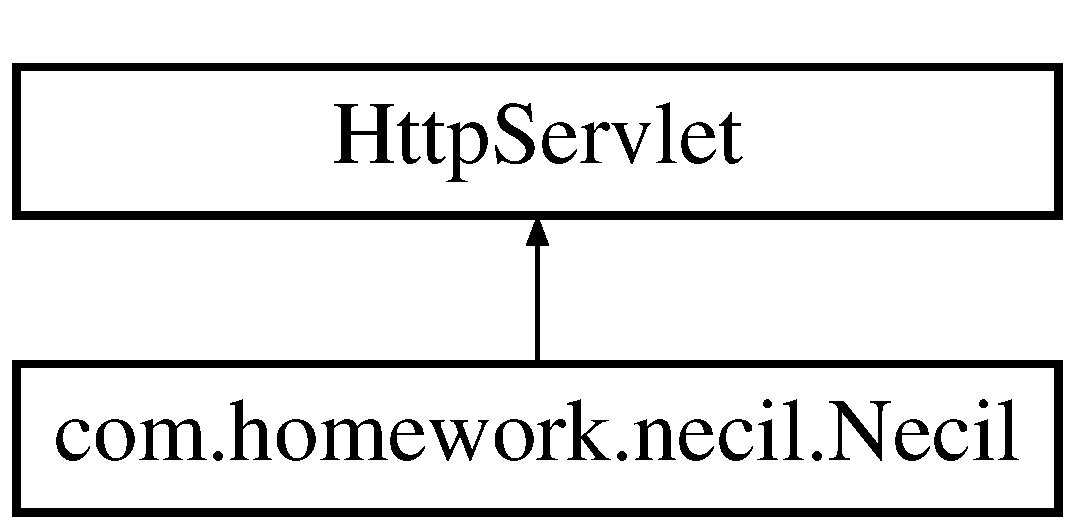
\includegraphics[height=2.000000cm]{classcom_1_1homework_1_1necil_1_1_necil}
\end{center}
\end{figure}
\subsection*{Public Member Functions}
\begin{DoxyCompactItemize}
\item 
\hyperlink{classcom_1_1homework_1_1necil_1_1_necil_a1b53c7e47f81edf92d25150a2ecfba5b}{Necil} ()
\end{DoxyCompactItemize}
\subsection*{Protected Member Functions}
\begin{DoxyCompactItemize}
\item 
void \hyperlink{classcom_1_1homework_1_1necil_1_1_necil_a91bd9db24f4e7cb4129e352f66cbdbbf}{do\+Get} (Http\+Servlet\+Request request, Http\+Servlet\+Response response)  throws Servlet\+Exception, I\+O\+Exception 
\item 
void \hyperlink{classcom_1_1homework_1_1necil_1_1_necil_a45030251ca10a28047d5aa5f4c381983}{do\+Post} (Http\+Servlet\+Request request, Http\+Servlet\+Response response)  throws Servlet\+Exception, I\+O\+Exception 
\end{DoxyCompactItemize}
\subsection*{Static Private Attributes}
\begin{DoxyCompactItemize}
\item 
static final long \hyperlink{classcom_1_1homework_1_1necil_1_1_necil_a6b86c82842a7ebb56f07f3367e084e76}{serial\+Version\+U\+ID} = 1L
\end{DoxyCompactItemize}


\subsection{Detailed Description}
Servlet implementation class \hyperlink{classcom_1_1homework_1_1necil_1_1_necil}{Necil} 

\subsection{Constructor \& Destructor Documentation}
\index{com\+::homework\+::necil\+::\+Necil@{com\+::homework\+::necil\+::\+Necil}!Necil@{Necil}}
\index{Necil@{Necil}!com\+::homework\+::necil\+::\+Necil@{com\+::homework\+::necil\+::\+Necil}}
\subsubsection[{\texorpdfstring{Necil()}{Necil()}}]{\setlength{\rightskip}{0pt plus 5cm}com.\+homework.\+necil.\+Necil.\+Necil (
\begin{DoxyParamCaption}
{}
\end{DoxyParamCaption}
)}\hypertarget{classcom_1_1homework_1_1necil_1_1_necil_a1b53c7e47f81edf92d25150a2ecfba5b}{}\label{classcom_1_1homework_1_1necil_1_1_necil_a1b53c7e47f81edf92d25150a2ecfba5b}
\begin{DoxySeeAlso}{See also}
Http\+Servlet\+::\+Http\+Servlet() 
\end{DoxySeeAlso}


\subsection{Member Function Documentation}
\index{com\+::homework\+::necil\+::\+Necil@{com\+::homework\+::necil\+::\+Necil}!do\+Get@{do\+Get}}
\index{do\+Get@{do\+Get}!com\+::homework\+::necil\+::\+Necil@{com\+::homework\+::necil\+::\+Necil}}
\subsubsection[{\texorpdfstring{do\+Get(\+Http\+Servlet\+Request request, Http\+Servlet\+Response response)}{doGet(HttpServletRequest request, HttpServletResponse response)}}]{\setlength{\rightskip}{0pt plus 5cm}void com.\+homework.\+necil.\+Necil.\+do\+Get (
\begin{DoxyParamCaption}
\item[{Http\+Servlet\+Request}]{request, }
\item[{Http\+Servlet\+Response}]{response}
\end{DoxyParamCaption}
) throws Servlet\+Exception, I\+O\+Exception\hspace{0.3cm}{\ttfamily [protected]}}\hypertarget{classcom_1_1homework_1_1necil_1_1_necil_a91bd9db24f4e7cb4129e352f66cbdbbf}{}\label{classcom_1_1homework_1_1necil_1_1_necil_a91bd9db24f4e7cb4129e352f66cbdbbf}
\begin{DoxySeeAlso}{See also}
Http\+Servlet\+::do\+Get(\+Http\+Servlet\+Request request, Http\+Servlet\+Response response) 
\end{DoxySeeAlso}
\index{com\+::homework\+::necil\+::\+Necil@{com\+::homework\+::necil\+::\+Necil}!do\+Post@{do\+Post}}
\index{do\+Post@{do\+Post}!com\+::homework\+::necil\+::\+Necil@{com\+::homework\+::necil\+::\+Necil}}
\subsubsection[{\texorpdfstring{do\+Post(\+Http\+Servlet\+Request request, Http\+Servlet\+Response response)}{doPost(HttpServletRequest request, HttpServletResponse response)}}]{\setlength{\rightskip}{0pt plus 5cm}void com.\+homework.\+necil.\+Necil.\+do\+Post (
\begin{DoxyParamCaption}
\item[{Http\+Servlet\+Request}]{request, }
\item[{Http\+Servlet\+Response}]{response}
\end{DoxyParamCaption}
) throws Servlet\+Exception, I\+O\+Exception\hspace{0.3cm}{\ttfamily [protected]}}\hypertarget{classcom_1_1homework_1_1necil_1_1_necil_a45030251ca10a28047d5aa5f4c381983}{}\label{classcom_1_1homework_1_1necil_1_1_necil_a45030251ca10a28047d5aa5f4c381983}
\begin{DoxySeeAlso}{See also}
Http\+Servlet\+::do\+Post(\+Http\+Servlet\+Request request, Http\+Servlet\+Response response) 
\end{DoxySeeAlso}


\subsection{Member Data Documentation}
\index{com\+::homework\+::necil\+::\+Necil@{com\+::homework\+::necil\+::\+Necil}!serial\+Version\+U\+ID@{serial\+Version\+U\+ID}}
\index{serial\+Version\+U\+ID@{serial\+Version\+U\+ID}!com\+::homework\+::necil\+::\+Necil@{com\+::homework\+::necil\+::\+Necil}}
\subsubsection[{\texorpdfstring{serial\+Version\+U\+ID}{serialVersionUID}}]{\setlength{\rightskip}{0pt plus 5cm}final long com.\+homework.\+necil.\+Necil.\+serial\+Version\+U\+ID = 1L\hspace{0.3cm}{\ttfamily [static]}, {\ttfamily [private]}}\hypertarget{classcom_1_1homework_1_1necil_1_1_necil_a6b86c82842a7ebb56f07f3367e084e76}{}\label{classcom_1_1homework_1_1necil_1_1_necil_a6b86c82842a7ebb56f07f3367e084e76}


The documentation for this class was generated from the following file\+:\begin{DoxyCompactItemize}
\item 
src/com/homework/necil/\hyperlink{_necil_8java}{Necil.\+java}\end{DoxyCompactItemize}

\hypertarget{classcom_1_1homework_1_1salih_1_1_salih}{}\section{com.\+homework.\+salih.\+Salih Class Reference}
\label{classcom_1_1homework_1_1salih_1_1_salih}\index{com.\+homework.\+salih.\+Salih@{com.\+homework.\+salih.\+Salih}}
Inheritance diagram for com.\+homework.\+salih.\+Salih\+:\begin{figure}[H]
\begin{center}
\leavevmode
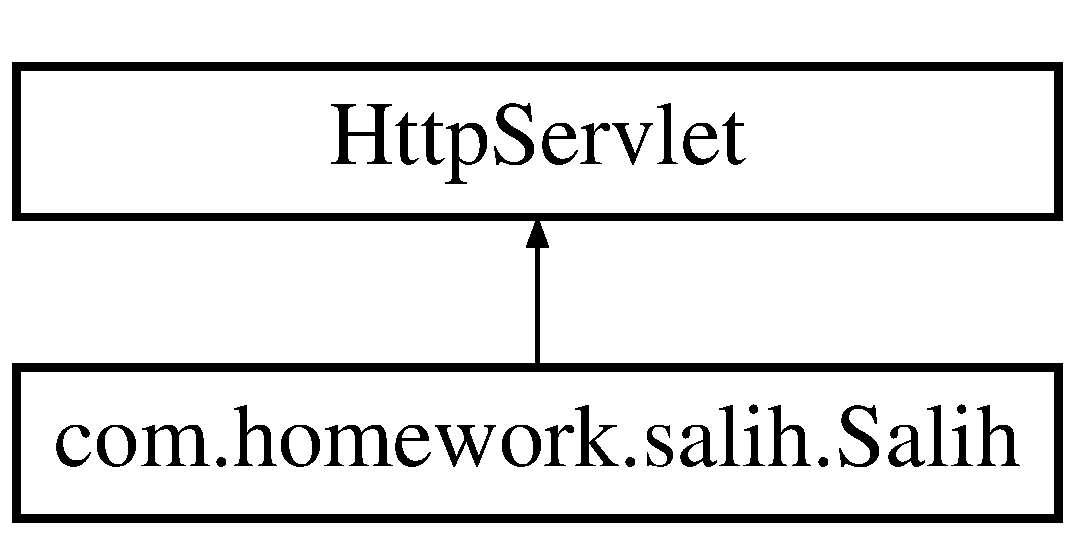
\includegraphics[height=2.000000cm]{classcom_1_1homework_1_1salih_1_1_salih}
\end{center}
\end{figure}
\subsection*{Public Member Functions}
\begin{DoxyCompactItemize}
\item 
\hyperlink{classcom_1_1homework_1_1salih_1_1_salih_a5a5cf5ea6350c6e886b31b07cab5a1ed}{Salih} ()
\end{DoxyCompactItemize}
\subsection*{Protected Member Functions}
\begin{DoxyCompactItemize}
\item 
void \hyperlink{classcom_1_1homework_1_1salih_1_1_salih_ae1a91aa8ab82a6be558a0f677af54ca5}{do\+Get} (Http\+Servlet\+Request request, Http\+Servlet\+Response response)  throws Servlet\+Exception, I\+O\+Exception 
\item 
void \hyperlink{classcom_1_1homework_1_1salih_1_1_salih_a12876a5d48986f78bf4f4f43a2c8bc07}{do\+Post} (Http\+Servlet\+Request request, Http\+Servlet\+Response response)  throws Servlet\+Exception, I\+O\+Exception 
\end{DoxyCompactItemize}
\subsection*{Static Private Attributes}
\begin{DoxyCompactItemize}
\item 
static final long \hyperlink{classcom_1_1homework_1_1salih_1_1_salih_a06003a300306fccbe0a10e15ee6fb247}{serial\+Version\+U\+ID} = 1L
\end{DoxyCompactItemize}


\subsection{Detailed Description}
Servlet implementation class \hyperlink{classcom_1_1homework_1_1salih_1_1_salih}{Salih} 

\subsection{Constructor \& Destructor Documentation}
\index{com\+::homework\+::salih\+::\+Salih@{com\+::homework\+::salih\+::\+Salih}!Salih@{Salih}}
\index{Salih@{Salih}!com\+::homework\+::salih\+::\+Salih@{com\+::homework\+::salih\+::\+Salih}}
\subsubsection[{\texorpdfstring{Salih()}{Salih()}}]{\setlength{\rightskip}{0pt plus 5cm}com.\+homework.\+salih.\+Salih.\+Salih (
\begin{DoxyParamCaption}
{}
\end{DoxyParamCaption}
)}\hypertarget{classcom_1_1homework_1_1salih_1_1_salih_a5a5cf5ea6350c6e886b31b07cab5a1ed}{}\label{classcom_1_1homework_1_1salih_1_1_salih_a5a5cf5ea6350c6e886b31b07cab5a1ed}
\begin{DoxySeeAlso}{See also}
Http\+Servlet\+::\+Http\+Servlet() 
\end{DoxySeeAlso}


\subsection{Member Function Documentation}
\index{com\+::homework\+::salih\+::\+Salih@{com\+::homework\+::salih\+::\+Salih}!do\+Get@{do\+Get}}
\index{do\+Get@{do\+Get}!com\+::homework\+::salih\+::\+Salih@{com\+::homework\+::salih\+::\+Salih}}
\subsubsection[{\texorpdfstring{do\+Get(\+Http\+Servlet\+Request request, Http\+Servlet\+Response response)}{doGet(HttpServletRequest request, HttpServletResponse response)}}]{\setlength{\rightskip}{0pt plus 5cm}void com.\+homework.\+salih.\+Salih.\+do\+Get (
\begin{DoxyParamCaption}
\item[{Http\+Servlet\+Request}]{request, }
\item[{Http\+Servlet\+Response}]{response}
\end{DoxyParamCaption}
) throws Servlet\+Exception, I\+O\+Exception\hspace{0.3cm}{\ttfamily [protected]}}\hypertarget{classcom_1_1homework_1_1salih_1_1_salih_ae1a91aa8ab82a6be558a0f677af54ca5}{}\label{classcom_1_1homework_1_1salih_1_1_salih_ae1a91aa8ab82a6be558a0f677af54ca5}
\begin{DoxySeeAlso}{See also}
Http\+Servlet\+::do\+Get(\+Http\+Servlet\+Request request, Http\+Servlet\+Response response) 
\end{DoxySeeAlso}
$<$ Our writer to type html codes \index{com\+::homework\+::salih\+::\+Salih@{com\+::homework\+::salih\+::\+Salih}!do\+Post@{do\+Post}}
\index{do\+Post@{do\+Post}!com\+::homework\+::salih\+::\+Salih@{com\+::homework\+::salih\+::\+Salih}}
\subsubsection[{\texorpdfstring{do\+Post(\+Http\+Servlet\+Request request, Http\+Servlet\+Response response)}{doPost(HttpServletRequest request, HttpServletResponse response)}}]{\setlength{\rightskip}{0pt plus 5cm}void com.\+homework.\+salih.\+Salih.\+do\+Post (
\begin{DoxyParamCaption}
\item[{Http\+Servlet\+Request}]{request, }
\item[{Http\+Servlet\+Response}]{response}
\end{DoxyParamCaption}
) throws Servlet\+Exception, I\+O\+Exception\hspace{0.3cm}{\ttfamily [protected]}}\hypertarget{classcom_1_1homework_1_1salih_1_1_salih_a12876a5d48986f78bf4f4f43a2c8bc07}{}\label{classcom_1_1homework_1_1salih_1_1_salih_a12876a5d48986f78bf4f4f43a2c8bc07}
\begin{DoxySeeAlso}{See also}
Http\+Servlet\+::do\+Post(\+Http\+Servlet\+Request request, Http\+Servlet\+Response response) 
\end{DoxySeeAlso}


\subsection{Member Data Documentation}
\index{com\+::homework\+::salih\+::\+Salih@{com\+::homework\+::salih\+::\+Salih}!serial\+Version\+U\+ID@{serial\+Version\+U\+ID}}
\index{serial\+Version\+U\+ID@{serial\+Version\+U\+ID}!com\+::homework\+::salih\+::\+Salih@{com\+::homework\+::salih\+::\+Salih}}
\subsubsection[{\texorpdfstring{serial\+Version\+U\+ID}{serialVersionUID}}]{\setlength{\rightskip}{0pt plus 5cm}final long com.\+homework.\+salih.\+Salih.\+serial\+Version\+U\+ID = 1L\hspace{0.3cm}{\ttfamily [static]}, {\ttfamily [private]}}\hypertarget{classcom_1_1homework_1_1salih_1_1_salih_a06003a300306fccbe0a10e15ee6fb247}{}\label{classcom_1_1homework_1_1salih_1_1_salih_a06003a300306fccbe0a10e15ee6fb247}


The documentation for this class was generated from the following file\+:\begin{DoxyCompactItemize}
\item 
src/com/homework/salih/\hyperlink{_salih_8java}{Salih.\+java}\end{DoxyCompactItemize}

\hypertarget{classcom_1_1homework_1_1aydin_1_1_sparql_aydin}{}\section{com.\+homework.\+aydin.\+Sparql\+Aydin Class Reference}
\label{classcom_1_1homework_1_1aydin_1_1_sparql_aydin}\index{com.\+homework.\+aydin.\+Sparql\+Aydin@{com.\+homework.\+aydin.\+Sparql\+Aydin}}
\subsection*{Public Member Functions}
\begin{DoxyCompactItemize}
\item 
\hyperlink{classcom_1_1homework_1_1aydin_1_1_sparql_aydin_a04b98701b1a3aa03dc2dd39502bd6155}{Sparql\+Aydin} ()
\item 
Vector$<$ \hyperlink{classcom_1_1homework_1_1aydin_1_1_model_aydin}{Model\+Aydin} $>$ \hyperlink{classcom_1_1homework_1_1aydin_1_1_sparql_aydin_ac7922de5a74ecd34598d1254699f17dd}{get\+Data} ()
\end{DoxyCompactItemize}
\subsection*{Private Attributes}
\begin{DoxyCompactItemize}
\item 
Result\+Set \hyperlink{classcom_1_1homework_1_1aydin_1_1_sparql_aydin_ac9dc7c9e7d107274e7034dc9448742b2}{results}
\item 
String \hyperlink{classcom_1_1homework_1_1aydin_1_1_sparql_aydin_ace2a9ff0a89fec9f4643590344c57e30}{squery}
\end{DoxyCompactItemize}


\subsection{Detailed Description}
Sparql query processing implementation class of \hyperlink{classcom_1_1homework_1_1aydin_1_1_aydin}{Aydin}. \begin{DoxyAuthor}{Author}
The Formal Boogieman 
\end{DoxyAuthor}


\subsection{Constructor \& Destructor Documentation}
\index{com\+::homework\+::aydin\+::\+Sparql\+Aydin@{com\+::homework\+::aydin\+::\+Sparql\+Aydin}!Sparql\+Aydin@{Sparql\+Aydin}}
\index{Sparql\+Aydin@{Sparql\+Aydin}!com\+::homework\+::aydin\+::\+Sparql\+Aydin@{com\+::homework\+::aydin\+::\+Sparql\+Aydin}}
\subsubsection[{\texorpdfstring{Sparql\+Aydin()}{SparqlAydin()}}]{\setlength{\rightskip}{0pt plus 5cm}com.\+homework.\+aydin.\+Sparql\+Aydin.\+Sparql\+Aydin (
\begin{DoxyParamCaption}
{}
\end{DoxyParamCaption}
)}\hypertarget{classcom_1_1homework_1_1aydin_1_1_sparql_aydin_a04b98701b1a3aa03dc2dd39502bd6155}{}\label{classcom_1_1homework_1_1aydin_1_1_sparql_aydin_a04b98701b1a3aa03dc2dd39502bd6155}
Constructor. Executes sparql query and saves the results. 

\subsection{Member Function Documentation}
\index{com\+::homework\+::aydin\+::\+Sparql\+Aydin@{com\+::homework\+::aydin\+::\+Sparql\+Aydin}!get\+Data@{get\+Data}}
\index{get\+Data@{get\+Data}!com\+::homework\+::aydin\+::\+Sparql\+Aydin@{com\+::homework\+::aydin\+::\+Sparql\+Aydin}}
\subsubsection[{\texorpdfstring{get\+Data()}{getData()}}]{\setlength{\rightskip}{0pt plus 5cm}Vector$<${\bf Model\+Aydin}$>$ com.\+homework.\+aydin.\+Sparql\+Aydin.\+get\+Data (
\begin{DoxyParamCaption}
{}
\end{DoxyParamCaption}
)}\hypertarget{classcom_1_1homework_1_1aydin_1_1_sparql_aydin_ac7922de5a74ecd34598d1254699f17dd}{}\label{classcom_1_1homework_1_1aydin_1_1_sparql_aydin_ac7922de5a74ecd34598d1254699f17dd}
Parses the sparql query result data into X\+ML format. \begin{DoxyReturn}{Returns}
X\+ML formatted query data vector. 
\end{DoxyReturn}


\subsection{Member Data Documentation}
\index{com\+::homework\+::aydin\+::\+Sparql\+Aydin@{com\+::homework\+::aydin\+::\+Sparql\+Aydin}!results@{results}}
\index{results@{results}!com\+::homework\+::aydin\+::\+Sparql\+Aydin@{com\+::homework\+::aydin\+::\+Sparql\+Aydin}}
\subsubsection[{\texorpdfstring{results}{results}}]{\setlength{\rightskip}{0pt plus 5cm}Result\+Set com.\+homework.\+aydin.\+Sparql\+Aydin.\+results\hspace{0.3cm}{\ttfamily [private]}}\hypertarget{classcom_1_1homework_1_1aydin_1_1_sparql_aydin_ac9dc7c9e7d107274e7034dc9448742b2}{}\label{classcom_1_1homework_1_1aydin_1_1_sparql_aydin_ac9dc7c9e7d107274e7034dc9448742b2}
\index{com\+::homework\+::aydin\+::\+Sparql\+Aydin@{com\+::homework\+::aydin\+::\+Sparql\+Aydin}!squery@{squery}}
\index{squery@{squery}!com\+::homework\+::aydin\+::\+Sparql\+Aydin@{com\+::homework\+::aydin\+::\+Sparql\+Aydin}}
\subsubsection[{\texorpdfstring{squery}{squery}}]{\setlength{\rightskip}{0pt plus 5cm}String com.\+homework.\+aydin.\+Sparql\+Aydin.\+squery\hspace{0.3cm}{\ttfamily [private]}}\hypertarget{classcom_1_1homework_1_1aydin_1_1_sparql_aydin_ace2a9ff0a89fec9f4643590344c57e30}{}\label{classcom_1_1homework_1_1aydin_1_1_sparql_aydin_ace2a9ff0a89fec9f4643590344c57e30}
{\bfseries Initial value\+:}
\begin{DoxyCode}
= \textcolor{stringliteral}{"PREFIX wd: <http://www.wikidata.org/entity/>"}
            + \textcolor{stringliteral}{"PREFIX wdt: <http://www.wikidata.org/prop/direct/>"}
            + \textcolor{stringliteral}{"PREFIX wikibase: <http://wikiba.se/ontology#>"}
            + \textcolor{stringliteral}{"PREFIX p: <http://www.wikidata.org/prop/>"}
            + \textcolor{stringliteral}{"PREFIX ps: <http://www.wikidata.org/prop/statement/>"}
            + \textcolor{stringliteral}{"PREFIX pq: <http://www.wikidata.org/prop/qualifier/>"}
            + \textcolor{stringliteral}{"PREFIX rdfs: <http://www.w3.org/2000/01/rdf-schema#>"}
            + \textcolor{stringliteral}{"PREFIX bd: <http://www.bigdata.com/rdf#>"}
            + \textcolor{stringliteral}{"SELECT ?p ?pLabel ?w ?wLabel "}
            + \textcolor{stringliteral}{"WHERE "}
            + \textcolor{stringliteral}{"\{"}
            + \textcolor{stringliteral}{"wd:Q30 p:P6/ps:P6 ?p ."}
            + \textcolor{stringliteral}{"?p wdt:P26 ?w ."}
            + \textcolor{stringliteral}{"SERVICE wikibase:label \{"}
            + \textcolor{stringliteral}{"bd:serviceParam wikibase:language \(\backslash\)"en\(\backslash\)" ."}
            + \textcolor{stringliteral}{"\}"}
            + \textcolor{stringliteral}{"\}"}
\end{DoxyCode}


The documentation for this class was generated from the following file\+:\begin{DoxyCompactItemize}
\item 
src/com/homework/aydin/\hyperlink{_sparql_aydin_8java}{Sparql\+Aydin.\+java}\end{DoxyCompactItemize}

\hypertarget{classcom_1_1homework_1_1yunus_1_1_sparql_yunus}{}\section{com.\+homework.\+yunus.\+Sparql\+Yunus Class Reference}
\label{classcom_1_1homework_1_1yunus_1_1_sparql_yunus}\index{com.\+homework.\+yunus.\+Sparql\+Yunus@{com.\+homework.\+yunus.\+Sparql\+Yunus}}
\subsection*{Public Member Functions}
\begin{DoxyCompactItemize}
\item 
\hyperlink{classcom_1_1homework_1_1yunus_1_1_sparql_yunus_ab4b87437911dc8b0287beb1376117064}{Sparql\+Yunus} ()
\item 
Vector$<$ \hyperlink{classcom_1_1homework_1_1yunus_1_1_model_yunus}{Model\+Yunus} $>$ \hyperlink{classcom_1_1homework_1_1yunus_1_1_sparql_yunus_a94b0fe53839f68e0001f3e5f414ec46a}{get\+Data} ()
\end{DoxyCompactItemize}
\subsection*{Static Public Member Functions}
\begin{DoxyCompactItemize}
\item 
static Document \hyperlink{classcom_1_1homework_1_1yunus_1_1_sparql_yunus_aba69854d3e0f548f888fb4291f2f9497}{load\+X\+M\+L\+From\+String} (String xml)  throws Exception 	
\end{DoxyCompactItemize}
\subsection*{Private Attributes}
\begin{DoxyCompactItemize}
\item 
Result\+Set \hyperlink{classcom_1_1homework_1_1yunus_1_1_sparql_yunus_a8501e4ed305ac8950893aa8b796a52ad}{results}
\item 
String \hyperlink{classcom_1_1homework_1_1yunus_1_1_sparql_yunus_ab6cecc25b9305e7ea928f09f380e6137}{squery}
\end{DoxyCompactItemize}


\subsection{Detailed Description}
Sparql implementation class of \hyperlink{classcom_1_1homework_1_1yunus_1_1_yunus}{Yunus}. \begin{DoxyAuthor}{Author}
\hyperlink{classcom_1_1homework_1_1yunus_1_1_yunus}{Yunus} 
\end{DoxyAuthor}


\subsection{Constructor \& Destructor Documentation}
\index{com\+::homework\+::yunus\+::\+Sparql\+Yunus@{com\+::homework\+::yunus\+::\+Sparql\+Yunus}!Sparql\+Yunus@{Sparql\+Yunus}}
\index{Sparql\+Yunus@{Sparql\+Yunus}!com\+::homework\+::yunus\+::\+Sparql\+Yunus@{com\+::homework\+::yunus\+::\+Sparql\+Yunus}}
\subsubsection[{\texorpdfstring{Sparql\+Yunus()}{SparqlYunus()}}]{\setlength{\rightskip}{0pt plus 5cm}com.\+homework.\+yunus.\+Sparql\+Yunus.\+Sparql\+Yunus (
\begin{DoxyParamCaption}
{}
\end{DoxyParamCaption}
)}\hypertarget{classcom_1_1homework_1_1yunus_1_1_sparql_yunus_ab4b87437911dc8b0287beb1376117064}{}\label{classcom_1_1homework_1_1yunus_1_1_sparql_yunus_ab4b87437911dc8b0287beb1376117064}
Constructor of the Class. By using jena library functions, takes the squery string and takes the result as a Result\+Set 

\subsection{Member Function Documentation}
\index{com\+::homework\+::yunus\+::\+Sparql\+Yunus@{com\+::homework\+::yunus\+::\+Sparql\+Yunus}!get\+Data@{get\+Data}}
\index{get\+Data@{get\+Data}!com\+::homework\+::yunus\+::\+Sparql\+Yunus@{com\+::homework\+::yunus\+::\+Sparql\+Yunus}}
\subsubsection[{\texorpdfstring{get\+Data()}{getData()}}]{\setlength{\rightskip}{0pt plus 5cm}Vector$<${\bf Model\+Yunus}$>$ com.\+homework.\+yunus.\+Sparql\+Yunus.\+get\+Data (
\begin{DoxyParamCaption}
{}
\end{DoxyParamCaption}
)}\hypertarget{classcom_1_1homework_1_1yunus_1_1_sparql_yunus_a94b0fe53839f68e0001f3e5f414ec46a}{}\label{classcom_1_1homework_1_1yunus_1_1_sparql_yunus_a94b0fe53839f68e0001f3e5f414ec46a}
Parses the data and returns it to the servlet. \begin{DoxyReturn}{Returns}
Model vector that holds the data. 
\end{DoxyReturn}
\index{com\+::homework\+::yunus\+::\+Sparql\+Yunus@{com\+::homework\+::yunus\+::\+Sparql\+Yunus}!load\+X\+M\+L\+From\+String@{load\+X\+M\+L\+From\+String}}
\index{load\+X\+M\+L\+From\+String@{load\+X\+M\+L\+From\+String}!com\+::homework\+::yunus\+::\+Sparql\+Yunus@{com\+::homework\+::yunus\+::\+Sparql\+Yunus}}
\subsubsection[{\texorpdfstring{load\+X\+M\+L\+From\+String(\+String xml)}{loadXMLFromString(String xml)}}]{\setlength{\rightskip}{0pt plus 5cm}static Document com.\+homework.\+yunus.\+Sparql\+Yunus.\+load\+X\+M\+L\+From\+String (
\begin{DoxyParamCaption}
\item[{String}]{xml}
\end{DoxyParamCaption}
) throws Exception\hspace{0.3cm}{\ttfamily [static]}}\hypertarget{classcom_1_1homework_1_1yunus_1_1_sparql_yunus_aba69854d3e0f548f888fb4291f2f9497}{}\label{classcom_1_1homework_1_1yunus_1_1_sparql_yunus_aba69854d3e0f548f888fb4291f2f9497}
Converts String X\+ML files to proper form that it can be parsed. 
\begin{DoxyParams}{Parameters}
{\em xml} & X\+ML as String \\
\hline
\end{DoxyParams}
\begin{DoxyReturn}{Returns}
document that is parsed. 
\end{DoxyReturn}

\begin{DoxyExceptions}{Exceptions}
{\em Exception} & \\
\hline
\end{DoxyExceptions}


\subsection{Member Data Documentation}
\index{com\+::homework\+::yunus\+::\+Sparql\+Yunus@{com\+::homework\+::yunus\+::\+Sparql\+Yunus}!results@{results}}
\index{results@{results}!com\+::homework\+::yunus\+::\+Sparql\+Yunus@{com\+::homework\+::yunus\+::\+Sparql\+Yunus}}
\subsubsection[{\texorpdfstring{results}{results}}]{\setlength{\rightskip}{0pt plus 5cm}Result\+Set com.\+homework.\+yunus.\+Sparql\+Yunus.\+results\hspace{0.3cm}{\ttfamily [private]}}\hypertarget{classcom_1_1homework_1_1yunus_1_1_sparql_yunus_a8501e4ed305ac8950893aa8b796a52ad}{}\label{classcom_1_1homework_1_1yunus_1_1_sparql_yunus_a8501e4ed305ac8950893aa8b796a52ad}
\index{com\+::homework\+::yunus\+::\+Sparql\+Yunus@{com\+::homework\+::yunus\+::\+Sparql\+Yunus}!squery@{squery}}
\index{squery@{squery}!com\+::homework\+::yunus\+::\+Sparql\+Yunus@{com\+::homework\+::yunus\+::\+Sparql\+Yunus}}
\subsubsection[{\texorpdfstring{squery}{squery}}]{\setlength{\rightskip}{0pt plus 5cm}String com.\+homework.\+yunus.\+Sparql\+Yunus.\+squery\hspace{0.3cm}{\ttfamily [private]}}\hypertarget{classcom_1_1homework_1_1yunus_1_1_sparql_yunus_ab6cecc25b9305e7ea928f09f380e6137}{}\label{classcom_1_1homework_1_1yunus_1_1_sparql_yunus_ab6cecc25b9305e7ea928f09f380e6137}
{\bfseries Initial value\+:}
\begin{DoxyCode}
= \textcolor{stringliteral}{"PREFIX wd: <http://www.wikidata.org/entity/>"}
            + \textcolor{stringliteral}{"PREFIX wdt: <http://www.wikidata.org/prop/direct/>"}
            + \textcolor{stringliteral}{"PREFIX wikibase: <http://wikiba.se/ontology#>"}
            + \textcolor{stringliteral}{"PREFIX p: <http://www.wikidata.org/prop/>"}
            + \textcolor{stringliteral}{"PREFIX ps: <http://www.wikidata.org/prop/statement/>"}
            + \textcolor{stringliteral}{"PREFIX pq: <http://www.wikidata.org/prop/qualifier/>"}
            + \textcolor{stringliteral}{"PREFIX rdfs: <http://www.w3.org/2000/01/rdf-schema#>"}
            + \textcolor{stringliteral}{"PREFIX bd: <http://www.bigdata.com/rdf#>"}
            + \textcolor{stringliteral}{"SELECT DISTINCT ?country ?countryLabel ?capitalLabel ?capital "}
            + \textcolor{stringliteral}{"WHERE"}
            + \textcolor{stringliteral}{"\{"}
            + \textcolor{stringliteral}{"?country wdt:P31 wd:Q3624078 ."}
            + \textcolor{stringliteral}{"OPTIONAL \{ ?country wdt:P36 ?capital \} ."}
            + \textcolor{stringliteral}{"SERVICE wikibase:label \{ bd:serviceParam wikibase:language \(\backslash\)"en\(\backslash\)" \}"}
            + \textcolor{stringliteral}{"\}"}
            + \textcolor{stringliteral}{"ORDER BY ?countryLabel"}
\end{DoxyCode}


The documentation for this class was generated from the following file\+:\begin{DoxyCompactItemize}
\item 
src/com/homework/yunus/\hyperlink{_sparql_yunus_8java}{Sparql\+Yunus.\+java}\end{DoxyCompactItemize}

\hypertarget{classcom_1_1homework_1_1yigit_1_1_yigit}{}\section{com.\+homework.\+yigit.\+Yigit Class Reference}
\label{classcom_1_1homework_1_1yigit_1_1_yigit}\index{com.\+homework.\+yigit.\+Yigit@{com.\+homework.\+yigit.\+Yigit}}
Inheritance diagram for com.\+homework.\+yigit.\+Yigit\+:\begin{figure}[H]
\begin{center}
\leavevmode
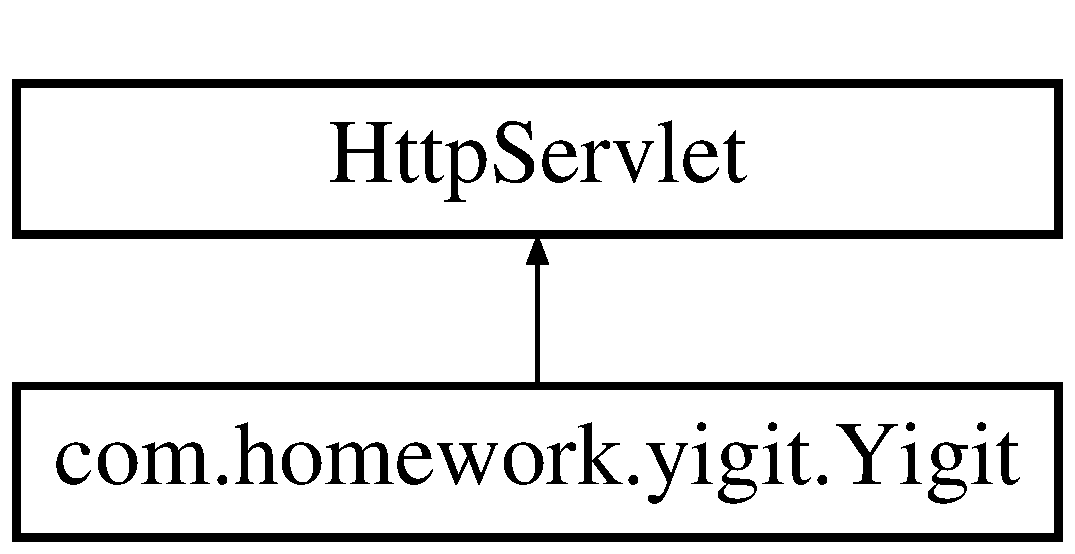
\includegraphics[height=2.000000cm]{classcom_1_1homework_1_1yigit_1_1_yigit}
\end{center}
\end{figure}
\subsection*{Public Member Functions}
\begin{DoxyCompactItemize}
\item 
\hyperlink{classcom_1_1homework_1_1yigit_1_1_yigit_aaea0e6d1611342b65620024b51b35a07}{Yigit} ()
\end{DoxyCompactItemize}
\subsection*{Protected Member Functions}
\begin{DoxyCompactItemize}
\item 
void \hyperlink{classcom_1_1homework_1_1yigit_1_1_yigit_a9fcdb429a94b0c565c1f82f2d672f8ff}{do\+Get} (Http\+Servlet\+Request request, Http\+Servlet\+Response response)  throws Servlet\+Exception, I\+O\+Exception 
\item 
void \hyperlink{classcom_1_1homework_1_1yigit_1_1_yigit_a8d4031c9f7529c9a2bebeb0240049faa}{do\+Post} (Http\+Servlet\+Request request, Http\+Servlet\+Response response)  throws Servlet\+Exception, I\+O\+Exception 
\end{DoxyCompactItemize}
\subsection*{Static Private Attributes}
\begin{DoxyCompactItemize}
\item 
static final long \hyperlink{classcom_1_1homework_1_1yigit_1_1_yigit_a3bef3a83f56c1f7bb2c1540d6f879f6a}{serial\+Version\+U\+ID} = 1L
\end{DoxyCompactItemize}


\subsection{Detailed Description}
Servlet implementation class \hyperlink{classcom_1_1homework_1_1yigit_1_1_yigit}{Yigit} 

\subsection{Constructor \& Destructor Documentation}
\index{com\+::homework\+::yigit\+::\+Yigit@{com\+::homework\+::yigit\+::\+Yigit}!Yigit@{Yigit}}
\index{Yigit@{Yigit}!com\+::homework\+::yigit\+::\+Yigit@{com\+::homework\+::yigit\+::\+Yigit}}
\subsubsection[{\texorpdfstring{Yigit()}{Yigit()}}]{\setlength{\rightskip}{0pt plus 5cm}com.\+homework.\+yigit.\+Yigit.\+Yigit (
\begin{DoxyParamCaption}
{}
\end{DoxyParamCaption}
)}\hypertarget{classcom_1_1homework_1_1yigit_1_1_yigit_aaea0e6d1611342b65620024b51b35a07}{}\label{classcom_1_1homework_1_1yigit_1_1_yigit_aaea0e6d1611342b65620024b51b35a07}
\begin{DoxySeeAlso}{See also}
Http\+Servlet\+::\+Http\+Servlet() 
\end{DoxySeeAlso}


\subsection{Member Function Documentation}
\index{com\+::homework\+::yigit\+::\+Yigit@{com\+::homework\+::yigit\+::\+Yigit}!do\+Get@{do\+Get}}
\index{do\+Get@{do\+Get}!com\+::homework\+::yigit\+::\+Yigit@{com\+::homework\+::yigit\+::\+Yigit}}
\subsubsection[{\texorpdfstring{do\+Get(\+Http\+Servlet\+Request request, Http\+Servlet\+Response response)}{doGet(HttpServletRequest request, HttpServletResponse response)}}]{\setlength{\rightskip}{0pt plus 5cm}void com.\+homework.\+yigit.\+Yigit.\+do\+Get (
\begin{DoxyParamCaption}
\item[{Http\+Servlet\+Request}]{request, }
\item[{Http\+Servlet\+Response}]{response}
\end{DoxyParamCaption}
) throws Servlet\+Exception, I\+O\+Exception\hspace{0.3cm}{\ttfamily [protected]}}\hypertarget{classcom_1_1homework_1_1yigit_1_1_yigit_a9fcdb429a94b0c565c1f82f2d672f8ff}{}\label{classcom_1_1homework_1_1yigit_1_1_yigit_a9fcdb429a94b0c565c1f82f2d672f8ff}
\begin{DoxySeeAlso}{See also}
Http\+Servlet\+::do\+Get(\+Http\+Servlet\+Request request, Http\+Servlet\+Response response) 
\end{DoxySeeAlso}
$<$ Our writer to type html codes \index{com\+::homework\+::yigit\+::\+Yigit@{com\+::homework\+::yigit\+::\+Yigit}!do\+Post@{do\+Post}}
\index{do\+Post@{do\+Post}!com\+::homework\+::yigit\+::\+Yigit@{com\+::homework\+::yigit\+::\+Yigit}}
\subsubsection[{\texorpdfstring{do\+Post(\+Http\+Servlet\+Request request, Http\+Servlet\+Response response)}{doPost(HttpServletRequest request, HttpServletResponse response)}}]{\setlength{\rightskip}{0pt plus 5cm}void com.\+homework.\+yigit.\+Yigit.\+do\+Post (
\begin{DoxyParamCaption}
\item[{Http\+Servlet\+Request}]{request, }
\item[{Http\+Servlet\+Response}]{response}
\end{DoxyParamCaption}
) throws Servlet\+Exception, I\+O\+Exception\hspace{0.3cm}{\ttfamily [protected]}}\hypertarget{classcom_1_1homework_1_1yigit_1_1_yigit_a8d4031c9f7529c9a2bebeb0240049faa}{}\label{classcom_1_1homework_1_1yigit_1_1_yigit_a8d4031c9f7529c9a2bebeb0240049faa}
\begin{DoxySeeAlso}{See also}
Http\+Servlet\+::do\+Post(\+Http\+Servlet\+Request request, Http\+Servlet\+Response response) 
\end{DoxySeeAlso}


\subsection{Member Data Documentation}
\index{com\+::homework\+::yigit\+::\+Yigit@{com\+::homework\+::yigit\+::\+Yigit}!serial\+Version\+U\+ID@{serial\+Version\+U\+ID}}
\index{serial\+Version\+U\+ID@{serial\+Version\+U\+ID}!com\+::homework\+::yigit\+::\+Yigit@{com\+::homework\+::yigit\+::\+Yigit}}
\subsubsection[{\texorpdfstring{serial\+Version\+U\+ID}{serialVersionUID}}]{\setlength{\rightskip}{0pt plus 5cm}final long com.\+homework.\+yigit.\+Yigit.\+serial\+Version\+U\+ID = 1L\hspace{0.3cm}{\ttfamily [static]}, {\ttfamily [private]}}\hypertarget{classcom_1_1homework_1_1yigit_1_1_yigit_a3bef3a83f56c1f7bb2c1540d6f879f6a}{}\label{classcom_1_1homework_1_1yigit_1_1_yigit_a3bef3a83f56c1f7bb2c1540d6f879f6a}


The documentation for this class was generated from the following file\+:\begin{DoxyCompactItemize}
\item 
src/com/homework/yigit/\hyperlink{_yigit_8java}{Yigit.\+java}\end{DoxyCompactItemize}

\hypertarget{classcom_1_1homework_1_1yunus_1_1_yunus}{}\section{com.\+homework.\+yunus.\+Yunus Class Reference}
\label{classcom_1_1homework_1_1yunus_1_1_yunus}\index{com.\+homework.\+yunus.\+Yunus@{com.\+homework.\+yunus.\+Yunus}}
Inheritance diagram for com.\+homework.\+yunus.\+Yunus\+:\begin{figure}[H]
\begin{center}
\leavevmode
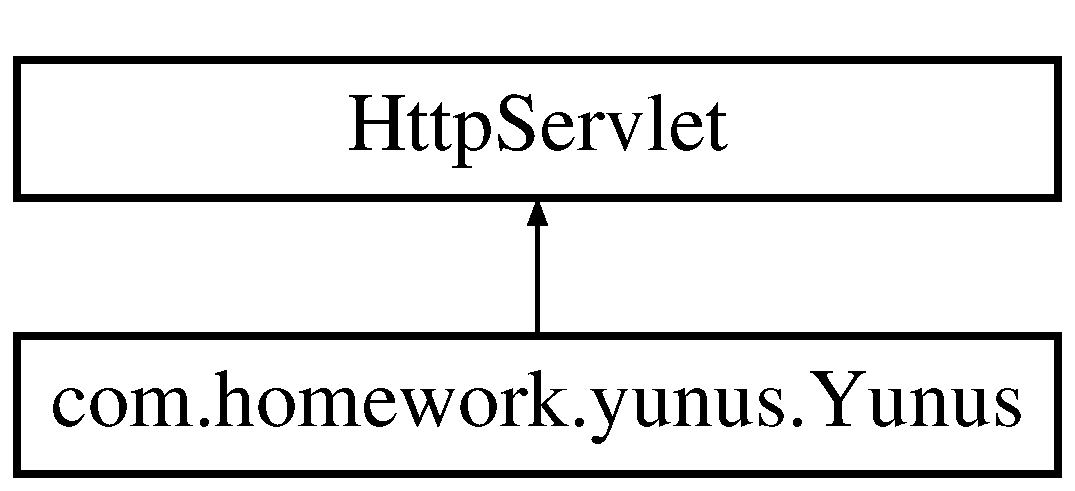
\includegraphics[height=2.000000cm]{classcom_1_1homework_1_1yunus_1_1_yunus}
\end{center}
\end{figure}
\subsection*{Public Member Functions}
\begin{DoxyCompactItemize}
\item 
\hyperlink{classcom_1_1homework_1_1yunus_1_1_yunus_a9d5871f9e874380b129c6dff31f1531b}{Yunus} ()
\end{DoxyCompactItemize}
\subsection*{Protected Member Functions}
\begin{DoxyCompactItemize}
\item 
void \hyperlink{classcom_1_1homework_1_1yunus_1_1_yunus_a2653e3f269da80881e2abfa6b30dc708}{do\+Get} (Http\+Servlet\+Request request, Http\+Servlet\+Response response)  throws Servlet\+Exception, I\+O\+Exception 
\item 
void \hyperlink{classcom_1_1homework_1_1yunus_1_1_yunus_abe7ecc6a6e297a44a50731348270ae17}{do\+Post} (Http\+Servlet\+Request req, Http\+Servlet\+Response resp)  throws Servlet\+Exception, I\+O\+Exception 
\end{DoxyCompactItemize}
\subsection*{Static Private Attributes}
\begin{DoxyCompactItemize}
\item 
static final long \hyperlink{classcom_1_1homework_1_1yunus_1_1_yunus_a135ed76b5ead6a58aa5f941be9477ed1}{serial\+Version\+U\+ID} = 1L
\end{DoxyCompactItemize}


\subsection{Detailed Description}
Servlet implementation of \hyperlink{classcom_1_1homework_1_1yunus_1_1_yunus}{Yunus}. \begin{DoxyAuthor}{Author}
\hyperlink{classcom_1_1homework_1_1yunus_1_1_yunus}{Yunus} 
\end{DoxyAuthor}


\subsection{Constructor \& Destructor Documentation}
\index{com\+::homework\+::yunus\+::\+Yunus@{com\+::homework\+::yunus\+::\+Yunus}!Yunus@{Yunus}}
\index{Yunus@{Yunus}!com\+::homework\+::yunus\+::\+Yunus@{com\+::homework\+::yunus\+::\+Yunus}}
\subsubsection[{\texorpdfstring{Yunus()}{Yunus()}}]{\setlength{\rightskip}{0pt plus 5cm}com.\+homework.\+yunus.\+Yunus.\+Yunus (
\begin{DoxyParamCaption}
{}
\end{DoxyParamCaption}
)}\hypertarget{classcom_1_1homework_1_1yunus_1_1_yunus_a9d5871f9e874380b129c6dff31f1531b}{}\label{classcom_1_1homework_1_1yunus_1_1_yunus_a9d5871f9e874380b129c6dff31f1531b}
\begin{DoxySeeAlso}{See also}
Http\+Servlet\+::\+Http\+Servlet() 
\end{DoxySeeAlso}


\subsection{Member Function Documentation}
\index{com\+::homework\+::yunus\+::\+Yunus@{com\+::homework\+::yunus\+::\+Yunus}!do\+Get@{do\+Get}}
\index{do\+Get@{do\+Get}!com\+::homework\+::yunus\+::\+Yunus@{com\+::homework\+::yunus\+::\+Yunus}}
\subsubsection[{\texorpdfstring{do\+Get(\+Http\+Servlet\+Request request, Http\+Servlet\+Response response)}{doGet(HttpServletRequest request, HttpServletResponse response)}}]{\setlength{\rightskip}{0pt plus 5cm}void com.\+homework.\+yunus.\+Yunus.\+do\+Get (
\begin{DoxyParamCaption}
\item[{Http\+Servlet\+Request}]{request, }
\item[{Http\+Servlet\+Response}]{response}
\end{DoxyParamCaption}
) throws Servlet\+Exception, I\+O\+Exception\hspace{0.3cm}{\ttfamily [protected]}}\hypertarget{classcom_1_1homework_1_1yunus_1_1_yunus_a2653e3f269da80881e2abfa6b30dc708}{}\label{classcom_1_1homework_1_1yunus_1_1_yunus_a2653e3f269da80881e2abfa6b30dc708}
Starting page of the application. \begin{DoxySeeAlso}{See also}
Http\+Servlet\+::do\+Get(\+Http\+Servlet\+Request request, Http\+Servlet\+Response response) 
\end{DoxySeeAlso}
$<$ Our writer to type html codes \index{com\+::homework\+::yunus\+::\+Yunus@{com\+::homework\+::yunus\+::\+Yunus}!do\+Post@{do\+Post}}
\index{do\+Post@{do\+Post}!com\+::homework\+::yunus\+::\+Yunus@{com\+::homework\+::yunus\+::\+Yunus}}
\subsubsection[{\texorpdfstring{do\+Post(\+Http\+Servlet\+Request req, Http\+Servlet\+Response resp)}{doPost(HttpServletRequest req, HttpServletResponse resp)}}]{\setlength{\rightskip}{0pt plus 5cm}void com.\+homework.\+yunus.\+Yunus.\+do\+Post (
\begin{DoxyParamCaption}
\item[{Http\+Servlet\+Request}]{req, }
\item[{Http\+Servlet\+Response}]{resp}
\end{DoxyParamCaption}
) throws Servlet\+Exception, I\+O\+Exception\hspace{0.3cm}{\ttfamily [protected]}}\hypertarget{classcom_1_1homework_1_1yunus_1_1_yunus_abe7ecc6a6e297a44a50731348270ae17}{}\label{classcom_1_1homework_1_1yunus_1_1_yunus_abe7ecc6a6e297a44a50731348270ae17}
Looks to the actions of the Servlet. Make methods work when buttons are pressed. $<$ Our writer to type html codes 

\subsection{Member Data Documentation}
\index{com\+::homework\+::yunus\+::\+Yunus@{com\+::homework\+::yunus\+::\+Yunus}!serial\+Version\+U\+ID@{serial\+Version\+U\+ID}}
\index{serial\+Version\+U\+ID@{serial\+Version\+U\+ID}!com\+::homework\+::yunus\+::\+Yunus@{com\+::homework\+::yunus\+::\+Yunus}}
\subsubsection[{\texorpdfstring{serial\+Version\+U\+ID}{serialVersionUID}}]{\setlength{\rightskip}{0pt plus 5cm}final long com.\+homework.\+yunus.\+Yunus.\+serial\+Version\+U\+ID = 1L\hspace{0.3cm}{\ttfamily [static]}, {\ttfamily [private]}}\hypertarget{classcom_1_1homework_1_1yunus_1_1_yunus_a135ed76b5ead6a58aa5f941be9477ed1}{}\label{classcom_1_1homework_1_1yunus_1_1_yunus_a135ed76b5ead6a58aa5f941be9477ed1}


The documentation for this class was generated from the following file\+:\begin{DoxyCompactItemize}
\item 
src/com/homework/yunus/\hyperlink{_yunus_8java}{Yunus.\+java}\end{DoxyCompactItemize}

\chapter{File Documentation}
\hypertarget{_aydin_8java}{}\section{src/com/homework/aydin/\+Aydin.java File Reference}
\label{_aydin_8java}\index{src/com/homework/aydin/\+Aydin.\+java@{src/com/homework/aydin/\+Aydin.\+java}}
\subsection*{Classes}
\begin{DoxyCompactItemize}
\item 
class \hyperlink{classcom_1_1homework_1_1aydin_1_1_aydin}{com.\+homework.\+aydin.\+Aydin}
\end{DoxyCompactItemize}
\subsection*{Packages}
\begin{DoxyCompactItemize}
\item 
package \hyperlink{namespacecom_1_1homework_1_1aydin}{com.\+homework.\+aydin}
\end{DoxyCompactItemize}

\hypertarget{_d_b_aydin_8java}{}\section{src/com/homework/aydin/\+D\+B\+Aydin.java File Reference}
\label{_d_b_aydin_8java}\index{src/com/homework/aydin/\+D\+B\+Aydin.\+java@{src/com/homework/aydin/\+D\+B\+Aydin.\+java}}
\subsection*{Classes}
\begin{DoxyCompactItemize}
\item 
class \hyperlink{classcom_1_1homework_1_1aydin_1_1_d_b_aydin}{com.\+homework.\+aydin.\+D\+B\+Aydin}
\end{DoxyCompactItemize}
\subsection*{Packages}
\begin{DoxyCompactItemize}
\item 
package \hyperlink{namespacecom_1_1homework_1_1aydin}{com.\+homework.\+aydin}
\end{DoxyCompactItemize}

\hypertarget{_model_aydin_8java}{}\section{src/com/homework/aydin/\+Model\+Aydin.java File Reference}
\label{_model_aydin_8java}\index{src/com/homework/aydin/\+Model\+Aydin.\+java@{src/com/homework/aydin/\+Model\+Aydin.\+java}}
\subsection*{Classes}
\begin{DoxyCompactItemize}
\item 
class \hyperlink{classcom_1_1homework_1_1aydin_1_1_model_aydin}{com.\+homework.\+aydin.\+Model\+Aydin}
\end{DoxyCompactItemize}
\subsection*{Packages}
\begin{DoxyCompactItemize}
\item 
package \hyperlink{namespacecom_1_1homework_1_1aydin}{com.\+homework.\+aydin}
\end{DoxyCompactItemize}

\hypertarget{_sparql_aydin_8java}{}\section{src/com/homework/aydin/\+Sparql\+Aydin.java File Reference}
\label{_sparql_aydin_8java}\index{src/com/homework/aydin/\+Sparql\+Aydin.\+java@{src/com/homework/aydin/\+Sparql\+Aydin.\+java}}
\subsection*{Classes}
\begin{DoxyCompactItemize}
\item 
class \hyperlink{classcom_1_1homework_1_1aydin_1_1_sparql_aydin}{com.\+homework.\+aydin.\+Sparql\+Aydin}
\end{DoxyCompactItemize}
\subsection*{Packages}
\begin{DoxyCompactItemize}
\item 
package \hyperlink{namespacecom_1_1homework_1_1aydin}{com.\+homework.\+aydin}
\end{DoxyCompactItemize}

\hypertarget{_db_denizalp_8java}{}\section{src/com/homework/denizalp/\+Db\+Denizalp.java File Reference}
\label{_db_denizalp_8java}\index{src/com/homework/denizalp/\+Db\+Denizalp.\+java@{src/com/homework/denizalp/\+Db\+Denizalp.\+java}}
\subsection*{Classes}
\begin{DoxyCompactItemize}
\item 
class \hyperlink{classcom_1_1homework_1_1denizalp_1_1_db_denizalp}{com.\+homework.\+denizalp.\+Db\+Denizalp}
\end{DoxyCompactItemize}
\subsection*{Packages}
\begin{DoxyCompactItemize}
\item 
package \hyperlink{namespacecom_1_1homework_1_1denizalp}{com.\+homework.\+denizalp}
\end{DoxyCompactItemize}

\hypertarget{_denizalp_8java}{}\section{src/com/homework/denizalp/\+Denizalp.java File Reference}
\label{_denizalp_8java}\index{src/com/homework/denizalp/\+Denizalp.\+java@{src/com/homework/denizalp/\+Denizalp.\+java}}
\subsection*{Classes}
\begin{DoxyCompactItemize}
\item 
class \hyperlink{classcom_1_1homework_1_1denizalp_1_1_denizalp}{com.\+homework.\+denizalp.\+Denizalp}
\end{DoxyCompactItemize}
\subsection*{Packages}
\begin{DoxyCompactItemize}
\item 
package \hyperlink{namespacecom_1_1homework_1_1denizalp}{com.\+homework.\+denizalp}
\end{DoxyCompactItemize}

\hypertarget{_home_8java}{}\section{src/com/homework/home/\+Home.java File Reference}
\label{_home_8java}\index{src/com/homework/home/\+Home.\+java@{src/com/homework/home/\+Home.\+java}}
\subsection*{Classes}
\begin{DoxyCompactItemize}
\item 
class \hyperlink{classcom_1_1homework_1_1home_1_1_home}{com.\+homework.\+home.\+Home}
\end{DoxyCompactItemize}
\subsection*{Packages}
\begin{DoxyCompactItemize}
\item 
package \hyperlink{namespacecom_1_1homework_1_1home}{com.\+homework.\+home}
\end{DoxyCompactItemize}

\hypertarget{_kubra_8java}{}\section{src/com/homework/kubra/\+Kubra.java File Reference}
\label{_kubra_8java}\index{src/com/homework/kubra/\+Kubra.\+java@{src/com/homework/kubra/\+Kubra.\+java}}
\subsection*{Classes}
\begin{DoxyCompactItemize}
\item 
class \hyperlink{classcom_1_1homework_1_1kubra_1_1_kubra}{com.\+homework.\+kubra.\+Kubra}
\end{DoxyCompactItemize}
\subsection*{Packages}
\begin{DoxyCompactItemize}
\item 
package \hyperlink{namespacecom_1_1homework_1_1kubra}{com.\+homework.\+kubra}
\end{DoxyCompactItemize}

\hypertarget{_necil_8java}{}\section{src/com/homework/necil/\+Necil.java File Reference}
\label{_necil_8java}\index{src/com/homework/necil/\+Necil.\+java@{src/com/homework/necil/\+Necil.\+java}}
\subsection*{Classes}
\begin{DoxyCompactItemize}
\item 
class \hyperlink{classcom_1_1homework_1_1necil_1_1_necil}{com.\+homework.\+necil.\+Necil}
\end{DoxyCompactItemize}
\subsection*{Packages}
\begin{DoxyCompactItemize}
\item 
package \hyperlink{namespacecom_1_1homework_1_1necil}{com.\+homework.\+necil}
\end{DoxyCompactItemize}

\hypertarget{_salih_8java}{}\section{src/com/homework/salih/\+Salih.java File Reference}
\label{_salih_8java}\index{src/com/homework/salih/\+Salih.\+java@{src/com/homework/salih/\+Salih.\+java}}
\subsection*{Classes}
\begin{DoxyCompactItemize}
\item 
class \hyperlink{classcom_1_1homework_1_1salih_1_1_salih}{com.\+homework.\+salih.\+Salih}
\end{DoxyCompactItemize}
\subsection*{Packages}
\begin{DoxyCompactItemize}
\item 
package \hyperlink{namespacecom_1_1homework_1_1salih}{com.\+homework.\+salih}
\end{DoxyCompactItemize}

\hypertarget{_yigit_8java}{}\section{src/com/homework/yigit/\+Yigit.java File Reference}
\label{_yigit_8java}\index{src/com/homework/yigit/\+Yigit.\+java@{src/com/homework/yigit/\+Yigit.\+java}}
\subsection*{Classes}
\begin{DoxyCompactItemize}
\item 
class \hyperlink{classcom_1_1homework_1_1yigit_1_1_yigit}{com.\+homework.\+yigit.\+Yigit}
\end{DoxyCompactItemize}
\subsection*{Packages}
\begin{DoxyCompactItemize}
\item 
package \hyperlink{namespacecom_1_1homework_1_1yigit}{com.\+homework.\+yigit}
\end{DoxyCompactItemize}

\hypertarget{_db_yunus_8java}{}\section{src/com/homework/yunus/\+Db\+Yunus.java File Reference}
\label{_db_yunus_8java}\index{src/com/homework/yunus/\+Db\+Yunus.\+java@{src/com/homework/yunus/\+Db\+Yunus.\+java}}
\subsection*{Classes}
\begin{DoxyCompactItemize}
\item 
class \hyperlink{classcom_1_1homework_1_1yunus_1_1_db_yunus}{com.\+homework.\+yunus.\+Db\+Yunus}
\end{DoxyCompactItemize}
\subsection*{Packages}
\begin{DoxyCompactItemize}
\item 
package \hyperlink{namespacecom_1_1homework_1_1yunus}{com.\+homework.\+yunus}
\end{DoxyCompactItemize}

\hypertarget{_model_yunus_8java}{}\section{src/com/homework/yunus/\+Model\+Yunus.java File Reference}
\label{_model_yunus_8java}\index{src/com/homework/yunus/\+Model\+Yunus.\+java@{src/com/homework/yunus/\+Model\+Yunus.\+java}}
\subsection*{Classes}
\begin{DoxyCompactItemize}
\item 
class \hyperlink{classcom_1_1homework_1_1yunus_1_1_model_yunus}{com.\+homework.\+yunus.\+Model\+Yunus}
\end{DoxyCompactItemize}
\subsection*{Packages}
\begin{DoxyCompactItemize}
\item 
package \hyperlink{namespacecom_1_1homework_1_1yunus}{com.\+homework.\+yunus}
\end{DoxyCompactItemize}

\hypertarget{_sparql_yunus_8java}{}\section{src/com/homework/yunus/\+Sparql\+Yunus.java File Reference}
\label{_sparql_yunus_8java}\index{src/com/homework/yunus/\+Sparql\+Yunus.\+java@{src/com/homework/yunus/\+Sparql\+Yunus.\+java}}
\subsection*{Classes}
\begin{DoxyCompactItemize}
\item 
class \hyperlink{classcom_1_1homework_1_1yunus_1_1_sparql_yunus}{com.\+homework.\+yunus.\+Sparql\+Yunus}
\end{DoxyCompactItemize}
\subsection*{Packages}
\begin{DoxyCompactItemize}
\item 
package \hyperlink{namespacecom_1_1homework_1_1yunus}{com.\+homework.\+yunus}
\end{DoxyCompactItemize}

\hypertarget{_yunus_8java}{}\section{src/com/homework/yunus/\+Yunus.java File Reference}
\label{_yunus_8java}\index{src/com/homework/yunus/\+Yunus.\+java@{src/com/homework/yunus/\+Yunus.\+java}}
\subsection*{Classes}
\begin{DoxyCompactItemize}
\item 
class \hyperlink{classcom_1_1homework_1_1yunus_1_1_yunus}{com.\+homework.\+yunus.\+Yunus}
\end{DoxyCompactItemize}
\subsection*{Packages}
\begin{DoxyCompactItemize}
\item 
package \hyperlink{namespacecom_1_1homework_1_1yunus}{com.\+homework.\+yunus}
\end{DoxyCompactItemize}

%--- End generated contents ---

% Index
\backmatter
\newpage
\phantomsection
\clearemptydoublepage
\addcontentsline{toc}{chapter}{Index}
\printindex

\end{document}
